\begin{center}
{\textbf{ಅಥ ದ್ವಿತೀಯೋऽಧ್ಯಾಯಃ ।}\\}
\end{center}
ಸಂಜಯ ಉವಾಚ ।\\
\slcol{\Index{ತಂ ತಥಾ ಕೃಪಯಾವಿಷ್ಟ}ಮಶ್ರುಪೂರ್ಣಾಕುಲೇಕ್ಷಣಮ್ ।\\
ವಿಷೀದಂತಮಿದಂ ವಾಕ್ಯಮುವಾಚ ಮಧುಸೂದನಃ ॥ ೧ ॥}
\cquote{ಸಂಜಯನು ಹೇಳಿದನು,  ಧೃತರಾಷ್ಟ್ರ ಮಹಾರಾಜ ಕೇಳು. 
ಈ ಪ್ರಕಾರ ಕಣ್ಣಿನಲ್ಲಿ ನೀರು ತುಂಬಿ ದುಃಖಿಸುತ್ತಿರುವ  ಅರ್ಜುನನನ್ನು ನೋಡಿ ಮಧುಸೂದನನು ಕೃಪೆಯಿಂದ ಈ ವಿಧವಾಗಿ ಹೇಳಿದನು.\\}
\slcol{ಶ್ರಿ\!\char"0CD5ಭಗವಾನುವಾಚ।\\
\Index{ಕುತಸ್ತ್ವಾ ಕಶ್ಮಲಮಿದಂ} ವಿಷಮೇ ಸಮುಪಸ್ಥಿತಮ್ ।\\
ಅನಾರ್ಯಜುಷ್ಟಮಸ್ವರ್ಗ್ಯಮಕೀರ್ತಿಕರಮರ್ಜುನ ॥ ೨ ॥}
\cquote{ಹೇ ಅರ್ಜುನಾ ! ಆರ್ಯರಿಗೆ  ಯೋಗ್ಯವಲ್ಲದ, ನರಕದಾಯಕವಾದ, ಅಪಕೀರ್ತಿಕರವಾದ ಈ ನೀಚ ವೃತ್ತಿ ಈ ಸಂಕಟಕಾಲದಲ್ಲಿ ನಿನಗೆ ಹೇಗೆ ಆವರಿಸಿತು?\\}
\slcol{\Index{ಕ್ಲೈಬ್ಯಂ ಮಾ ಸ್ಮ ಗಮಃ }ಪಾರ್ಥ ನೈತತ್ತ್ವಯ್ಯುಪಪದ್ಯತೇ ।\\
ಕ್ಷುದ್ರಂ ಹೃದಯದೌರ್ಬಲ್ಯಂ ತ್ಯಕ್ತ್ವೋತ್ತಿಷ್ಠ ಪರಂತಪ ॥ ೩ ॥}
\cquote{ಪಾರ್ಥಾ! ಈ ಹೇಡಿತನವನ್ನು ಬಿಡು. ಇದು ನಿನಗೆ ಯೋಗ್ಯವಾದುದಲ್ಲ. ಹೇ ಶತ್ರುಮರ್ದನಾ! ತುಚ್ಛವಾದ ಮನೋದೌರ್ಬಲ್ಯವನ್ನು ತ್ಯಜಿಸಿ ಯುದ್ಧಕ್ಕೆ ಏಳು.\\}
\slcol{ಅರ್ಜುನ ಉವಾಚ ।\\
\Index{ಕಥಂ ಭೀಷ್ಮಮಹಂ} ಸಂಖ್ಯೇ ದ್ರೋಣಂ ಚ ಮಧುಸೂದನ ।\\
ಇಷುಭಿಃ ಪ್ರತಿಯೋತ್ಸ್ಯಾಮಿ ಪೂಜಾರ್ಹಾವರಿಸೂದನ ॥ ೪ ॥}
\cquote{ಅರ್ಜುನನು ಹೀಗೆಂದನು, ಹೇ ಮಧುಸೂದನ! ನನ್ನಿಂದ ಪೂಜೆಗೊಳ್ಳುವುದಕ್ಕೆ ತಕ್ಕವರಾದ ಭೀಷ್ಮ ದ್ರೋಣರನ್ನು  ಯುದ್ಧದಲ್ಲಿ ಎದುರಿಸಿ ಬಾಣಗಳಿಂದ ಹೇಗೆ ಹೊಡೆಯಲಿ?}

\newpage
\begin{mananam}{\mananamfont{ಮನನ ಶ್ಲೋಕ - ೨, ೩}}
\small \mananatext ನನ್ನ ಮನಸ್ಸು ಸ್ವಾನುಕಂಪಕದಲ್ಲಿಯೇ ಕೇಂದ್ರೀಕೃತವಾಗಿದೆಯೇ? ನನ್ನ ಕೆಲವು ಬಾಹ್ಯ ಪರಿಸ್ಥಿತಿಗಳು ಮತ್ತು ಆಂತರಿಕ ಪ್ರಚೋದನೆಗಳು ನನ್ನ ಶಕ್ತಿಯನ್ನು ಕುಂಠಿತ ಮಾಡುವ ಬಲವನ್ನು ಹೊಂದಿವೆಯೇ ಹಾಗೂ ಈ ಶಕ್ತಿ ಮತ್ತು ಪ್ರಚೋದನೆಗಳಿಗೆ, ನನ್ನ ದುರ್ಬಲತೆಯಿಂದಾಗಿ ದಾಸನಾಗಿದ್ದೇನೆಯೇ? ಗುರುಗಳು, ಹಿತೈಷಿಗಳು ಮಾಡಿದ ಸದುಪದೇಶಗಳನ್ನೂ ಸಹಿತ ಅಳವಡಿಸಿಕೊಳ್ಳಲಾರದಷ್ಟು ವೇದನಾಶೀಲನಾಗಿ, ಮನದ ದ್ವಾರವನ್ನು ಮುಚ್ಚಿಬಿಟ್ಟಿದ್ದೇನೆಯೇ?\\
ದುರ್ಬಲತೆಯಿಂದಾಗಿ ಅಥವಾ ಹತಾಷೆಯಿಂದಾಗಿ, ಜೀವನದಲ್ಲಿಯ ಒಳ್ಳೆಯ ಗುರಿ ಮತ್ತು ನಿರ್ಣಯಗಳನ್ನು, ಗಾಢವಾಗಿ ಯೋಚಿಸದೇ, ಸುಲಭವಾಗಿ ತೊರೆದುಬಿಡುತ್ತೇನೆಯೇ? ನನ್ನ ಜೀವನದಲ್ಲಿ, ನನ್ನ ಗುರಿಯಾದ, ಧನಾತ್ಮಕ ಬದಲಾವಣೆ ತರಲು ಏನು ಮಾಡಬೇಕೆಂಬುದರ ಬಗ್ಗೆ ನನಗೆ ಅರಿವಿದೆಯೇ? ಹಾಗೆ ಮಾಡಿದ ಬದಲಾವಣೆಯನ್ನು ಬಿಡದೆಲೇ, ಜೀವನದಲ್ಲಿ ಸ್ಥಿರಪಡಿಸುವ ಛಲವಿದೆಯೇ?
\end{mananam}
\WritingHand\enspace\textbf{ಆತ್ಮ ವಿಮರ್ಶೆ}\\
\begin{inspiration}{\mananamfont ಸ್ಪೂರ್ತಿ}
\small \mananatext ಸವಾಲುಗಳನ್ನು ಎದುರಿಸಲು ನೀವು ಎಂದಿಗೂ ದುರ್ಬಲರಲ್ಲ. ನಮ್ಮ ಜೀವನದಲ್ಲಿ,  ಬುದ್ಧಿ, ಮನಸ್ಸು, ದೇಹದ ಬಗ್ಗೆ ಯಾವುದೇ ಪರೀಕ್ಷೆಯನ್ನು ಆ ಭಗವಂತ ನಮಗೆ ಕೊಡುವುದು, ನಮ್ಮ ಬಲ ವೃದ್ಧಿಸಿ ನಮ್ಮನ್ನು ಸಕ್ಷಮ ಮಾಡುವುದಕ್ಕಾಗಿಯೇ ಹೊರತು,  ನಮ್ಮನ್ನು ತೊಂದರೆಗೀಡುಮಾಡುವುದಕ್ಕಲ್ಲ; ಅಲ್ಲದೇ, ನಮಗೆ ಸಹಿಸಿಕೊಳ್ಳಲು ಇರುವ ಶಕ್ತಿಯಷ್ಟೇ ಪರೀಕ್ಷೆಗಳನ್ನು ಒಡ್ಡುತ್ತಾನೆ. ಯಾವುದೇ ತರಹದ ಪ್ರಲೋಭನೆ, ಸ್ವಯಂ ಅನುಕಂಪ ಮತ್ತು ಅನುಮಾನಗಳಿಗೆ ಆಸ್ಪದ ಕೊಡಬೇಡಿ. ಜೀವನದ ಅತ್ಯುನ್ನತ ಗುರಿ ಮತ್ತು ಆಕಾಂಕ್ಷೆಗಳೊಂದಿಗೆ ಮುಂದುವರೆಯಿರಿ. ನೀವು ಒಂದು ದೃಢ ಸಂಕಲ್ಪ ಮಾಡಿದಾಗ, ಇಡೀ ಬ್ರಹ್ಮಾಂಡದ ಎಲ್ಲಾ ಸಕಾರಾತ್ಮಕ ಶಕ್ತಿಗಳೂ ನಿಮ್ಮನ್ನು ಬಲಪಡಿಸಿ ಬೆಂಬಲಿಸುತ್ತವೆ.
\end{inspiration}
\newpage

\slcol{\Index{ಗುರೂನಹತ್ವಾ ಹಿ} ಮಹಾನುಭಾವಾನ್ಶ್ರೇಯೋ ಭೋಕ್ತುಂ ಭೈಕ್ಷ್ಯಮಪೀಹ ಲೋಕೇ ।\\
ಹತ್ವಾರ್ಥಕಾಮಾಂಸ್ತು ಗುರುನಿಹೈವ ಭುಂಜೀಯ ಭೋಗಾನ್ ರುಧಿರಪ್ರದಿಗ್ಧಾನ್ ॥ ೫ ॥}
\cquote{ಮಹಾತ್ಮರಾದ ಗುರುಗಳನ್ನು ಕೊಲ್ಲುವ ಬದಲು ಈ ಲೋಕದಲ್ಲಿ ತಿರಿದು ತಿನ್ನುವುದಾದರೂ ಮೇಲು. ಅವರನ್ನು ವಧಿಸಿದರೆ ಅವರ ರಕ್ತದಿಂದ ಸಿಕ್ತವಾದ ಅರ್ಥಕಾಮಭೋಗಗಳನ್ನೇ  ಇಲ್ಲಿ ತಿನ್ನಬೇಕಾಗುತ್ತದೆ.\\}
\slcol{\Index{ನ ಚೈತದ್ವಿದ್ಮಃ ಕತರನ್ನೋ} ಗರೀಯೋ ಯದ್ವಾ \\ಜಯೇಮ ಯದಿ ವಾ ನೋ ಜಯೇಯುಃ ।\\
ಯಾನೇವ ಹತ್ವಾ ನ ಜಿಜೀವಿಷಾಮಸ್ತೇऽವಸ್ಥಿತಾಃ \\ಪ್ರಮುಖೇ ಧಾರ್ತರಾಷ್ಟ್ರಾಃ ॥ ೬ ॥}
\cquote{ಯಾವುದು ಸರಿಯೋ ಯಾವುದು ತಪ್ಪೋ ಗೊತ್ತಿಲ್ಲ. ನಾವು ಗೆಲ್ಲುವೆವೂ ಅಥವಾ ಅವರೇ ನಮ್ಮನ್ನು ಗೆಲ್ಲುವರೋ ಅದೂ ಗೊತ್ತಿಲ್ಲ. ಯಾರನ್ನು ಕೊಂದು ನಾವು ಬದುಕ ಬಯಸುವುದಿಲ್ಲವೋ ಅಂತಹ ಕೌರವರೇ ಎದುರಿಗೆ ನಿಂತಿದ್ದಾರೆ.\\}
\slcol{\Index{ಕಾರ್ಪಣ್ಯದೋಷೋಪ}ಹತಸ್ವಭಾವಃ \\ಪೃಚ್ಛಾಮಿ ತ್ವಾಂ ಧರ್ಮಸಂಮೂಢಚೇತಾಃ ।\\
ಯಚ್ಛ್ರೇಯಃ ಸ್ಯಾನ್ನಿಶ್ಚಿತಂ ಬ್ರೂಹಿ ತನ್ಮೇ \\ಶಿಷ್ಯಸ್ತೇऽಹಂ ಶಾಧಿ ಮಾಂ ತ್ವಾಂ ಪ್ರಪನ್ನಮ್ ॥ ೭ ॥}
\cquote{ಮನೋದೌರ್ಬಲ್ಯ ದೋಷದಿಂದ ನನ್ನ ಸ್ವಾಭಾವಿಕ ಶಕ್ತಿಯು ನಷ್ಟವಾಗಿದೆ. ಧರ್ಮಾಧರ್ಮದ ಬಗೆಗೆ ಮನಸ್ಸು ನಿರ್ಧರಿಸಲಾರದಾಗಿದೆ. ಆದ್ದರಿಂದ ನಿನ್ನನ್ನು ಕೇಳಿಕೊಳ್ಳುತ್ತೇನೆ, ಯಾವುದು ಸರಿ ಎಂಬುದನ್ನು ನೀನೆ ನನಗೆ ತಿಳಿ ಹೇಳಬೇಕು. ನಾನು ನಿನಗೆ ಶಿಷ್ಯನು. ಶರಣು ಬಂದಿರುವ ನನಗೆ ನೀನೇ ದಾರಿ ತೋರಬೇಕು.\\}
\slcol{\Index{ನ ಹಿ ಪ್ರಪಶ್ಯಾಮಿ ಮಮಾಪ}ನುದ್ಯಾದ್ಯಚ್ಛೋಕಮು\\ಚ್ಛೋಷಣಮಿಂದ್ರಿಯಾಣಾಮ್ ।\\
ಅವಾಪ್ಯ ಭೂಮಾವಸಪತ್ನಮೃದ್ಧಂ \\ರಾಜ್ಯಂ ಸುರಾಣಾಮಪಿ ಚಾಧಿಪತ್ಯಮ್ ॥ ೮ ॥}
\cquote{ಶತ್ರುಗಳಿಲ್ಲದ  ಸಮೃದ್ಧವಾದ ಇಡಿಯ ಭೂಮಂಡಲದ ಒಡೆತನ ಅಥವಾ ದೇವಲೋಕದ ಒಡೆತನವೇ ದೊರೆತರೂ ನನ್ನ ಇಂದ್ರಿಯಗಳನ್ನೆಲ್ಲ ಸೊರಗಿಸುವ ಈ ದುಃಖವನ್ನು ಕಳೆದೀತೆಂದು ನನಗೆ ಕಾಣುವುದಿಲ್ಲ.\\}
\slcol{ಸಂಜಯ ಉವಾಚ ।\\
\Index{ಏವಮುಕ್ತ್ವಾ ಹೃಷೀಕೇಶಂ} ಗುಡಾಕೇಶಃ ಪರಂತಪ ।\\
ನ ಯೋತ್ಸ್ಯ ಇತಿ ಗೋವಿಂದಮುಕ್ತ್ವಾ ತೂಷ್ಣೀಂ ಬಭೂವ ಹ ॥ ೯ ॥}
\cquote{ಸಂಜಯನು ಹೇಳಿದನು, ಶತ್ರು ಗಳನ್ನು ಗದಗುಟ್ಟಿಸುವ ಅರ್ಜುನನು ಕೃಷ್ಣನನ್ನು ಕುರಿತು ಹೀಗೆ ಹೇಳಿ, ನಾನು ಕಾದಲಾರೆ ಎಂದು ಸುಮ್ಮನಾದನು.\\}
\newpage

\begin{mananam}{\mananamfont ಮನನ ಶ್ಲೋಕ - ೭}
\small \mananatext ನಮ್ಮ ಜೀವನದಲ್ಲಿ ಸರಿಯಾದ ತಿಳುವಳಿಕೆಯಿಂದ, ನಮ್ಮಲ್ಲಿರುವ ಮಿತಿ ಮತ್ತು  ದೌರ್ಬಲ್ಯದ  ಅರಿವನ್ನು, ಅಧ್ಯಾತ್ಮ ಲಕ್ಷಣಗಳಾದ ಪವಿತ್ರ ಭಾವನೆ ಮತ್ತು ನಮ್ರತೆಯಾಗಿ ರೂಪಾಂತರಿಸಬಹುದು. \\
‘ನನಗೆ ಎಲ್ಲವೂ ಗೊತ್ತಿಲ್ಲ ಅಥವಾ ನನ್ನ ಬುದ್ಧಿಮತ್ತೆಗೆ ನಿಲುಕದ್ದು ಬಹಳಷ್ಟು ಇವೆ ’ ಎಂದು ತಿಳಿದುಕೊಳ್ಳುವಷ್ಟು ನಾನು ವಿನಮ್ರನಾಗಿದ್ದೇನೆಯೇ? ನಾನು, ನನ್ನ ಜೀವನದಲ್ಲಿ, ಋಷಿಮುನಿಗಳ ಮತ್ತು ಆಧ್ಯಾತ್ಮಿಕ ಗುರುಗಳ, ಜೀವನ  ರೂಪಾಂತರಿಸುವ ಸತ್ಯಕ್ಕೆ, ನನ್ನ ಹೃದಯದ ದ್ವಾರವನ್ನು ತೆರೆದಿಡಬಲ್ಲೆನೇ? ಆ ಪರಮಸತ್ಯವನ್ನು ಆಹ್ವಾನಿಸಬಲ್ಲೆನೇ?
\end{mananam}
\WritingHand\enspace\textbf{ಆತ್ಮ ವಿಮರ್ಶೆ}
\begin{inspiration}{\mananamfont ಸ್ಪೂರ್ತಿ}
\small \mananatext ‘ಶಿಷ್ಯನು ಸಿದ್ಧವಾದಾಗ (ಪಾತ್ರಕ್ಕೆ ಅರ್ಹನಾದಾಗ), ಅವನ ಬಳಿ ಗುರು ಬಂದೇ ಬರುತ್ತಾನೆ’ ಎಂಬುದು ಎಲ್ಲಾ ಅಧ್ಯಾತ್ಮಿಕ ಅನ್ವೇಷಕರಿಗೆ ಹೇಳುವ ಗಾದೆಯಾಗಿದೆ. ಇಲ್ಲಿ ಸಿದ್ಧವಾಗಿರುವುದು ಎಂದರೆ, ಸಮಯವಾಧಾರಿತ ಅಳತೆಗೋಲಲ್ಲ ಆದರೆ, ಶಿಷ್ಯನ ಮಾನಸಿಕ ಸ್ಥಿತಿಗಳಾದ ಮುಕ್ತಮನಸ್ಸು, ಗ್ರಹಿಕೆಯ ಶಕ್ತಿ ಹಾಗೂ, ಸ್ವೀಕೃತ ಹೃದಯವೇ ಆಗಿದೆ. ನಿಜವಾದ ನಮ್ರತೆಯು ನಮ್ಮ ದೌರ್ಬಲ್ಯವಲ್ಲ ಅದು ಶ್ರೇಷ್ಠತೆ; ಇದು ದೈವತ್ವದ ದ್ವಾರವನ್ನು ತೆರೆಯುತ್ತದೆ!
\end{inspiration}
\newpage


\slcol{\Index{ತಮುವಾಚ ಹೃಷೀಕೇಶಃ} ಪ್ರಹಸನ್ನಿವ ಭಾರತ ।\\
ಸೇನಯೋರುಭಯೋರ್ಮಧ್ಯೇ ವಿಷೀದಂತಮಿದಂ ವಚಃ ॥ ೧೦ ॥}
\cquote{ದೃತರಾಷ್ಟ್ರನೇ, ಎರಡು ದಂಡುಗಳ ನಡುವೆ ವ್ಯಥೆಗೊಳ್ಳುತ್ತಿರುವ ಅರ್ಜುನನ್ನು ಕುರಿತು ಕೃಷ್ಣನು ಮುಗುಳು ನಗುತ್ತಲೇ ಹೀಗೆ ಹೇಳಿದನು.\\}
\slcol{ಶ್ರಿ\!\char"0CD5ಭಗವಾನುವಾಚ ।\\
\Index{ಅಶೋಚ್ಯಾನನ್ವಶೋಚಸ್ತ್ವಂ} ಪ್ರಙ್ಞಾವಾದಾಂಶ್ಚ ಭಾಷಸೇ ।\\
ಗತಾಸೂನಗತಾಸೂಂಶ್ಚ ನಾನುಶೋಚಂತಿ ಪಂಡಿತಾಃ ॥ ೧೧ ॥}
\cquote{ಶ್ರಿ\!\char"0CD5 ಭಗವಂತನು ಹೇಳಿದನು,\\
ನೀನು ಯಾರಿಗಾಗಿ ಅಳಬಾರದೊ ಅವರಿಗಾಗಿ ಅಳುತ್ತಿ, ಜಾಣನಂತೆ ಮಾತುಗಳನ್ನು ಆಡುತ್ತಿ, ತಿಳಿದವರು ಸತ್ತವರಿಗಾಗಲಿ ಸಾಯುವವರಿಗಾಗಲಿ ಅಳುವುದಿಲ್ಲ.\\}
\slcol{\Index{ನ ತ್ವೇವಾಹಂ ಜಾತು} ನಾಸಂ ನ ತ್ವಂ ನೇಮೇ ಜನಾಧಿಪಾಃ ।\\
ನ ಚೈವ ನ ಭವಿಷ್ಯಾಮಃ ಸರ್ವೇ ವಯಮತಃ ಪರಮ್ ॥ ೧೨ ॥}
\cquote{ನಾನು, ನೀನು, ಈ ಅರಸರು ಹಿಂದೆಂದೂ ಇಲ್ಲವೆಂದಾದುದಿಲ್ಲ. ಮುಂದೆಯೂ ನಾವೆಲ್ಲರೂ ಇಲ್ಲವಾಗಲಾರೆವು.\\}
\slcol{\Index{ದೇಹಿನೋऽಸ್ಮಿನ್ಯಥಾ ದೇಹೇ} ಕೌಮಾರಂ ಯೌವನಂ ಜರಾ ।\\
ತಥಾ ದೇಹಾಂತರಪ್ರಾಪ್ತಿರ್ಧೀರಸ್ತತ್ರ ನ ಮುಹ್ಯತಿ ॥ ೧೩ ॥}
\cquote{ಈ ಶರೀರಕ್ಕೆ ಬಾಲ್ಯ, ಯೌವನ, ವಾರ್ಧಕ್ಯ ಅವಸ್ಥೆಗಳು ಕ್ರಮವಾಗಿ ಬರುವಂತೆ, ಆತ್ಮನಿಗೆ ಆಯಾ ದೇಹಗಳು ಬರುತ್ತಿರುತ್ತವೆ. ಈ ವಿಷಯದಲ್ಲಿ ಧೀರನು ಮೋಹಕ್ಕೆ ಒಳಗಾಗುವುದಿಲ್ಲ.\\}
\slcol{\Index{ಮಾತ್ರಾಸ್ಪರ್ಶಾಸ್ತು ಕೌಂತೇಯ} ಶೀತೋಷ್ಣಸುಖದುಃಖದಾಃ ।\\
ಆಗಮಾಪಾಯಿನೋऽನಿತ್ಯಾಸ್ತಾಂಸ್ತಿತಿಕ್ಷಸ್ವ ಭಾರತ ॥ ೧೪ ॥}
\cquote{ಕುಂತಿಪುತ್ರ, ಇಂದ್ರಿಯಗಳು ವಿಷಯಗಳೊಂದಿಗೆ ಕೂಡಿದಾಗ ಶೀತೋಷ್ಣ ಸುಖ ದುಃಖಗಳು ಸಂಭವಿಸುತ್ತವೆ. ಆ ಕೂಡಿಕೆ ಸ್ಥಿರವಲ್ಲ. ಬಂದು ಹೋಗುತ್ತಿರುತ್ತವೆ. ಆದುದರಿಂದ ಭಾರತ ವೀರನೇ ಸಹಿಸಿಕೋ.\\}
\slcol{\Index{ಯಂ ಹಿ ನ ವ್ಯಥಯಂತ್ಯೇತೇ} ಪುರುಷಂ ಪುರುಷರ್ಷಭ ।\\
ಸಮದುಃಖಸುಖಂ ಧೀರಂ ಸೋऽಮೃತತ್ವಾಯ ಕಲ್ಪತೇ ॥ ೧೫ ॥}
\cquote{ ಹೇ ಪುರುಷವರ್ಯಾ, ಸುಖ-ದುಃಖಗಳಲ್ಲಿ ಒಂದೇ ತೆರನಾಗಿರುವ ಯಾವ ಧೀರನನ್ನು ವಿಷಯ ಸಂಯೋಗಗಳು ವ್ಯಥೆಗೊಳಿಸುವುದಿಲ್ಲವೋ, ಅವನು ಮೋಕ್ಷಕ್ಕೆ ಯೋಗ್ಯನಾಗುತ್ತಾನೆ.\\}

\newpage
\begin{mananam}{\mananamfont ಮನನ ಶ್ಲೋಕ - ೧೧}
\small \mananatext ನನ್ನ ಅಂತಃಸ್ಪುರಣೆ ಮತ್ತು ಬುದ್ಧಿವಂತಿಕೆಯ ಮೇಲೆ ನಾನು ನಿಲುವುಗಳನ್ನು ತೆಗೆದುಕೊಳ್ಳುತ್ತೇನೆಯೇ? ಅಥವಾ ‘ನನ್ನ ನಿಲುವುಗಳೇ ಸರಿ’ ಎಂದು ಅದನ್ನು ಅನುಮೋದಿಸಲು ಅಧಿಕೃತ ಬೋಧನೆಗಳನ್ನು ದುರುಪಯೋಗಪಡಿಸಿಕೊಳ್ಳುತ್ತೇನೆಯೇ? ಜೀವನದ ಕಷ್ಟಕರ ಸನ್ನಿವೇಶಗಳಲ್ಲಿ, ಕಷ್ಟಕರವಾದರೂ, ದೃಢವಾದ ನಿಲುವನ್ನು ಧೈರ್ಯವಾಗಿ ತೆಗೆದುಕೊಳ್ಳುತ್ತೇನೆಯೇ? ಅಥವಾ, ತಪ್ಪಿಸಿಕೊಳ್ಳುವ, ಸುಲಭದ ಹಾದಿಯನ್ನು ಹಿಡಿಯುತ್ತೇನೆಯೇ?\\
ಮರಣಿಸಿದವರ ಚೈತನ್ಯವನ್ನು ನಾನು, ಜೀವಂತವಾಗಿ ಹೇಗೆ ಇಡಬಲ್ಲೆ? ನನ್ನ ಪ್ರಿಯಜನರ ಸದ್ಗುಣಗಳ ಬಗ್ಗೆ ನನಗೆ ಗಮನವಿದೆಯೇ ಹಾಗೂ ಅವುಗಳನ್ನು ಕಲಿಯುತ್ತೇನೆಯೇ? ಮತ್ತು, ಅವರ ಮರಣದ ನಂತರ, ಅವರ ಜೀವನದ ಮೌಲ್ಯಗಳನ್ನು, ನನ್ನ ಜೀವನದಲ್ಲಿ ಅಳವಡಿಸಿಕೊಳ್ಳುವುದರ ಮೂಲಕ ಅವರ ಆತ್ಮವನ್ನು ಗೌರವಿಸುತ್ತೇನೆಯೇ?
\end{mananam}
\WritingHand\enspace\textbf{ಆತ್ಮ ವಿಮರ್ಶೆ}
\begin{inspiration}{\mananamfont ಸ್ಪೂರ್ತಿ}
\small \mananatext ನುಡಿದಂತೆ ನಡೆಯುವುದು ಮಾನಸಿಕ ಶಕ್ತಿಯ ಚಿಹ್ನೆ; ಶಾಸ್ತ್ರಗಳನ್ನು ಉಲ್ಲೇಖಿಸಿ ಅಥವಾ ಇತರರ ಉದಾಹರಣೆ ಕೊಟ್ಟು, ತನ್ನ ನಿಶ್ಕ್ರಿಯತೆಗೆ ನಾನಾಕಾರಣಕೊಟ್ಟು ಸಮರ್ಥಿಸಿಕೊಳ್ಳುವುದು, ದೌರ್ಬಲ್ಯದ ಕುರುಹು.
\end{inspiration}
\newpage

\begin{mananam}{\mananamfont ಮನನ ಶ್ಲೋಕ - ೧೩}
\small \mananatext ನನ್ನ ಜೀವನದಲ್ಲಿ ಬದಲಾವಣೆಗಳನ್ನು ವಿರೋಧಿಸುತ್ತೇನೆಯೇ? ನನ್ನಲ್ಲಿ ಉತ್ತಮ ಆರೋಗ್ಯ ಮತ್ತು ಯೌವ್ವನದ ಶಕ್ತಿ ಇರುವಾಗ ಮನಸ್ಸು ಉಲ್ಲಾಸವಾಗಿರುತ್ತದೆ, ಮತ್ತು ಶಕ್ತಿ ಕುಂದಿದಾಗ, ಅನಾರೋಗ್ಯ ಇರುವಾಗ ಮನಸ್ಸು ಅಸಮಾಧಾನಗೊಳ್ಳುತ್ತದೆಯೇ? ಈ ಪ್ರಕೃತಿಯಲ್ಲಿ ಎಲ್ಲವೂ ನಿರಂತರ ಬದಲಾವಣೆಗೆ ಒಳಪಟ್ಟಿದೆ ಎಂದು ತಿಳಿದೂ ಕೂಡ ನನಗೆ, ದೈಹಿಕ ಬದಲಾವಣೆಗಳಾದಾಗ, ಮನಸ್ಸು ವಿಚಲಿತವಾಗದೇ, ದೃಢವಾಗಿಟ್ಟುಕೊಳ್ಳುವುದರ ಪ್ರಾಮುಖ್ಯತೆ ತಿಳಿದಿದೆಯೇ? ನನ್ನ ದೈಹಿಕ ಲಕ್ಷಣಗಳನ್ನು ಇತರರಿಗೆ ಹೋಲಿಸಿಕೊಂಡು, ಖೇದ ಅಥವಾ ಹೆಮ್ಮೆ ಪಡುತ್ತೇನೆಯೇ? ನನ್ನ ದೈಹಿಕ ಲಕ್ಷಣಗಳು ಮತ್ತು ವಯಸ್ಸಿನ ಆಧಾರದ ಮೇಲೆ ನನ್ನ ಜೀವನದಲ್ಲಿ ಮಿತಿಗಳನ್ನು, ನನ್ನ ಮೇಲೆ ನಾನು ಹೇರಿಕೊಳ್ಳುತ್ತೇನೆಯೇ?
\end{mananam}
\WritingHand\enspace\textbf{ಆತ್ಮ ವಿಮರ್ಶೆ}
\begin{inspiration}{\mananamfont ಸ್ಪೂರ್ತಿ}
\small \mananatext ಬಾಲ್ಯ, ಯೌವ್ವನ, ವೃದ್ಧಾಪ್ಯ ಈ ದೇಹದ ನೈಸರ್ಗಿಕ ಪ್ರಕ್ರಿಯೆಯಾಗಿದೆ. ಯೌವನದಲ್ಲಿರುವ ಸೌಂದರ್ಯವೇ ಸತ್ಯ ಮತ್ತು ಚಿರಂತನವಾಗಿರಬೇಕು ಎಂದು ಬಯಸಿದರೆ, ದುಃಖ ಖಚಿತ. ದೈಹಿಕ ಸೌಂದರ್ಯಕ್ಕಿಂತ ಮನಸ್ಸಿನ ನಿರ್ಮಲತೆ, ಶುದ್ಧತೆಯೇ ಶ್ರೇಷ್ಠ; ಬದಲಾವಣೆಯಾಗದೆ, ದೇಹದೊಂದಿಗಿರುವ ಆತ್ಮದ ಸೌಂದರ್ಯ, ಇದೆಲ್ಲದರಕ್ಕಿಂತಲೂ  ಅತ್ಯಂತ ಶ್ರೇಷ್ಠವಾಗಿದೆ.
 ಶಾಶ್ವತ ಸುಖವನ್ನರಸುವ ಮಾನವನು,  ಸದಾ ಬದಲಾಗುವ ತನ್ನ ದೈಹಿಕ ಸ್ಥಿತಿಯನ್ನು ಮೀರಿ, ಎಂದೂ ಬದಲಾಗದೇ ಇರುವ ಆತ್ಮದ ಬಗ್ಗೆ ಅರಿತುಕೊಳ್ಳಲೆಂದೇ, ಆ ಪರಮಾತ್ಮನು,  ಸದಾ ಬದಲಾವಣೆಗೆ ಒಳಪಡುವಂತೆಯೇ ಈ ದೇಹವನ್ನು ಕೌಶಲ್ಯದಿಂದ ವಿನ್ಯಾಸಮಾಡಿದ್ದಾನೆ!
\end{inspiration}
\newpage

\begin{mananam}{\mananamfont ಮನನ ಶ್ಲೋಕ - ೧೪}
\small \mananatext ನಮ್ಮ ದೇಹದಂತೆಯೇ ಮಾನಸಿಕ ಸ್ಥಿತಿಯೂ ಕೂಡಾ ಬದಲಾಗುತ್ತಲೇ ಇರುತ್ತದೆ. ನಾವು ನಮ್ಮ ಮಾನಸಿಕ ಸ್ಥಿತಿಯನ್ನು ಒಳ್ಳೆಯದು ಅಥವಾ ಕೆಟ್ಟದ್ದು ಎಂದು ನಿರ್ಣಯಿಸದೆ, ನಮ್ಮ ಮನಸ್ಸಿನ ಸ್ಥಿತಿಯ ಬಗ್ಗೆ ಅರಿಯಬಹುದೇ? (ಅಂದರೇ, ನನ್ನಲ್ಲೇಳುತ್ತಿರುವ ಮನಸ್ಸಿನ ಭಾವನೆಗಳಾದ, ಕೋಪ,  ಭಯ, ಸಂತೋಷ ಇತ್ಯಾದಿ.,) ಮನಸ್ಸಿನಲ್ಲಿ ಸುಳಿಯುವ ನಾನಾ ವಿಧವಾದ ಭಾವನೆಗಳ ಏರಿಳಿತಗಳು ಅಂದರೆ,ಕೋಪ, ಭಯ, ದುಃಖ ಅಥವಾ, ಉದ್ವೇಗ, ತೃಪ್ತಿ ಮತ್ತು ಸಂತೋಷ ಇವೆಲ್ಲದರ ಹಿಂದೆ ದೃಢವಾಗಿ ಮತ್ತು ಸೂಕ್ಷ್ಮವಾಗಿ, ಇರುವ ಹಿನ್ನೆಲೆಯ ಸುಳಿವನ್ನು ಗ್ರಹಿಸಬಲ್ಲೆನೇ?\\
ಎಂದಾದರೂ ನಾನು, ‘ನನ್ನ ತಾಳ್ಮೆಯ ಸೀಮೆ ಮುಗಿಯಿತು, ಇನ್ನು ಏನನ್ನೂ ನನ್ನಿಂದ ಸಹಿಸಲು ಸಾಧ್ಯವೇ ಇಲ್ಲ’ ಎಂಬ ಭಾವನೆಗೆ ಒಳಗಾಗಿದ್ದೇಯೇ? ನಾನು ಸುಲಭವಾಗಿ ತಾಳ್ಮೆ ಕಳೆದುಕೊಳ್ಳುತ್ತೇನೆಯೇ? ಸಿಡಿಮಿಡಿ ಗೊಳ್ಳುತ್ತೇನೆಯೇ? ಏತಕ್ಕೆ ಹೀಗೆ ಎಂದು, ಅದರ ಮೂಲ ಕಾರಣ ತಿಳಿಯಲು ಪ್ರೆರೇಪಿತನಾಗುತ್ತೇನೆಯೇ? ಹಾಗಿಲ್ಲದಿದ್ದಲ್ಲಿ,  ಬಹುಷಃ ನಾನು,  ಮನಸ್ಸಿನಲ್ಲಿ ಹಾದುಹೋಗುವ ವಿಚಾರಧಾರೆ, ಮನಸ್ಸಿನ ಏರಿಳಿತಗಳನ್ನೇ ಈ ಜೀವನದಲ್ಲಿ ಶಾಶ್ವತವೆಂದುಕೊಂಡಿದ್ದೇನೆ. 
\end{mananam}
\WritingHand\enspace\textbf{ಆತ್ಮ ವಿಮರ್ಶೆ}
\begin{inspiration}{\mananamfont ಸ್ಪೂರ್ತಿ}
\small \mananatext ಆ ಭಗವಂತನ ಭವ್ಯ ಚಿತ್ರಣವಾದ ನಮ್ಮ ಈ ಜೀವನದ ಸೃಷ್ಟಿಯು,ಹಳತಾದ, ನಿಶ್ಪ್ರಯೋಜಕವಾದ ನೆನಪುಗಳನ್ನೇ ಮೆಲಕುಹಾಕಲು ಅಲ್ಲ; ನಾವು ಮರೆತಿರುವ, ಆದರೆ, ಸಹಜವಾಗಿಯೇ ನಮ್ಮಲ್ಲಿರುವ ಆತ್ಮದ ಪ್ರಕೃತಿಯ ಬಗ್ಗೆ ತಿಳಿಯಲು ಎಂದಾಗಿದೆ. ಕ್ಷಣಿಕ ಸಂತೋಷ ಕೊಡುವ ಸಣ್ಣಪುಟ್ಟ ಅನುಭವಗಳಿಗೋಸ್ಕರ ಜೀವನದಲ್ಲಿ ಕೋರಿಕೆ ಇಡುತ್ತಾ ನಿಮ್ಮ ಸಮಯವನ್ನು ವ್ಯರ್ಥಮಾಡಬೇಡಿ.  ಶಾಶ್ವತ ಆನಂದವು ನಿಮ್ಮ ಜನ್ಮ ಸಿದ್ಧ ಹಕ್ಕು!
\end{inspiration}
\newpage

\begin{mananam}{\mananamfont ಮನನ ಶ್ಲೋಕ - ೧೫}
\small \mananatext ಸಂತೋಷವು ನನ್ನ ಅನುಭವಕ್ಕೆ ಬರುವುದು ಎಲ್ಲಿ?  ದುಃಖವು ನನ್ನ ಅನುಭವಕ್ಕೆ ಬರುವುದು ಎಲ್ಲಿ? ‘ಇವೆಲ್ಲವೂ ಕೇವಲ ಮಾನಸಿಕ ಸ್ಥಿತಿಗಳು’ ಎಂದು, ನೇರ ಒಳನೋಟದಲ್ಲಿ ನಾನು ಕಾಣಬಲ್ಲೆನೇ? ನಿಮ್ಮ ಜೀವನದಲ್ಲಿ ಕೆಲವೊಂದು ಸನ್ನಿವೇಶಗಳಲ್ಲಿ ಒಂದು ವಸ್ತು ನಿಮಗೆ ದುಃಖವನ್ನು ತರುತ್ತದೆ ಆದರೆ, ಅದೇ ವಸ್ತುವು ಬೇರೆಯವರಿಗೆ ಸಂತೋಷವನ್ನು ತರುತ್ತದೆ; ಅದು ಆಹಾರ, ಹವಾಮಾನ ಅಥವಾ ಇನ್ಯಾವುದೇ ಆಗಿರಬಹುದು ಎಂಬುದನ್ನು ಗಮನಿಸಿ; ಇದು ಹೀಗೇಕೆ? ಎಂಬುದರ ಬಗ್ಗೆ ವಿಚಾರ ಮಾಡಿ.ಇದಲ್ಲದೇ, ನಿಮ್ಮ ಮಾನಸಿಕ ಸ್ಥಿತಿಗಳ ಅರಿವಿನ ಬಗ್ಗೆಯೇ ನಿಮಗೆ ಜಾಗೃತಿ ಇದೆಯೇ?  ಈ ಜಾಗೃತಿ, ಕ್ಷಣ ಮಾತ್ರ ಮೂಡಿ ಮತ್ತೆ ಇಲ್ಲವಾಗುತ್ತದೆಯೇ? ಅಥವಾ, ಎಷ್ಟು ಸಮಯದ ವರೆವಿಗೂ ಈ ಜಾಗೃತಿಯನ್ನು ಹಿಡಿದಿಡಲು ಆಗುತ್ತದೆ ಎಂದು ಗಮನಿಸಿ.
\end{mananam}
\WritingHand\enspace\textbf{ಆತ್ಮ ವಿಮರ್ಶೆ}
\begin{inspiration}{\mananamfont ಸ್ಪೂರ್ತಿ}
\small \mananatext ಜೀವನದಲ್ಲಿ ಪ್ರತಿಯೊಂದು ಜೀವಿಗೂ ಸಾವಿನ ಭಯವಿರುವಂತೆಯೇ ಅಮರತ್ವವೂ ಕೂಡ ರಹಸ್ಯ ಬಯಕೆಯಾಗಿದೆ. ಆತ್ಮವು ಈ ದೇಹವನ್ನೂ ಮನಸ್ಸನ್ನೂ ಮೀರಿದುದಾಗಿದೆ ಎಂದು ಯಾರು ಅರಿತುಕೊಳ್ಳುವರೋ ಅವರು, ಬದಲಾಗುವ ಸ್ಥಿತಿಗಳಿಂದ ತೊಂದರೆಗೆ ಒಳಗಾಗುವುದಿಲ್ಲ. ಈ ತತ್ವವನ್ನು ತಿಳಿದ ವ್ಯಕ್ತಿಯು ಅಮರನಾಗುತ್ತಾನೆ. ಅವನು ಅಥವಾ ಅವಳು, 'ಮೂಲಭೂತವಾಗಿ, ತನ್ನ ಚೈತನ್ಯವು ಎಂದೆಂದಿಗೂ ಅಮರ' ಎಂದು ಅರಿತುಕೊಳ್ಳುತ್ತಾನೆ.
\end{inspiration}

\newpage
\slcol{\Index{ನಾಸತೋ ವಿದ್ಯತೇ ಭಾವೋ} ನಾಭಾವೋ ವಿದ್ಯತೇ ಸತಃ ।\\
ಉಭಯೋರಪಿ ದೃಷ್ಟೋऽಂತಸ್ತ್ವನಯೋಸ್ತತ್ತ್ವದರ್ಶಿಭಿಃ ॥ ೧೬ ॥}
\cquote{ ಇಲ್ಲದ ಅಸತ್ ಪದಾರ್ಥಕ್ಕೆ ಇರುವಿಕೆ ಇಲ್ಲ. ಇರುವ ಸದ್ ವಸ್ತುವಿಗೆ ಇಲ್ಲದಿರುವಿಕೆ ಇಲ್ಲ.  ಈ ಎರಡು ತತ್ವಗಳ ನಿರ್ಣಯವನ್ನು ತತ್ವಜ್ಞಾನಿಗಳು ಬಲ್ಲರು.\\}
\slcol{\Index{ಅವಿನಾಶಿ ತು ತದ್ವಿದ್ಧಿ} ಯೇನ ಸರ್ವಮಿದಂ ತತಮ್ ।\\
ವಿನಾಶಮವ್ಯಯಸ್ಯಾಸ್ಯ ನ ಕಶ್ಚಿತ್ಕರ್ತುಮರ್ಹತಿ ॥ ೧೭ ॥}
\cquote{ಈ ಸಮಸ್ತ ವಿಶ್ವವನ್ನು ತುಂಬಿಕೊಂಡಿರುವ ಆತ್ಮನು ನಾಶವಾಗುವವನಲ್ಲ. ಆ ಆತ್ಮನನ್ನು ನಾಶಗೊಳಿಸಲು ಯಾರೂ ಸಮರ್ಥರಲ್ಲ.\\}
\slcol{\Index{ಅಂತವಂತ ಇಮೇ ದೇಹಾ} ನಿತ್ಯಸ್ಯೋಕ್ತಾಃ ಶರೀರಿಣಃ ।\\
ಅನಾಶಿನೋऽಪ್ರಮೇಯಸ್ಯ ತಸ್ಮಾದ್ಯುಧ್ಯಸ್ವ ಭಾರತ ॥ ೧೮ ॥}
\cquote{ಈ ದೇಹಗಳು ಒಂದಲ್ಲ ಒಂದು ದಿನ ಹೋಗಲೇಬೇಕು. ಒಳಗಿರುವ ಜೀವ ಮಾತ್ರ ನಿತ್ಯ. ಪೂರ್ಣನಾದ ಭಗವಂತನಂತೆ ಅವನಿಗೂ ನಾಶವಿಲ್ಲ. ಆದ್ದರಿಂದ ನಿತ್ಯಪೂರ್ಣನಾದ ಭಗವಂತನ ಪೂಜೆಯಿಂದ, ಓ ಅರ್ಜುನ ಯುದ್ಧ ಮಾಡು.\\}
\slcol{\Index{ಯ ಏನಂ ವೇತ್ತಿ ಹಂತಾರಂ} ಯಶ್ಚೈನಂ ಮನ್ಯತೇ ಹತಮ್ ।\\
ಉಭೌ ತೌ ನ ವಿಜಾನೀತೋ ನಾಯಂ ಹಂತಿ ನ ಹನ್ಯತೇ ॥ ೧೯ ॥}
\cquote{ಜೀವನನ್ನು ಯಾರಾದರೂ ಕೊಲ್ಲಬಹುದು ಎಂದಾಗಲಿ ಆಗ ಜೀವ ಸಾಯುತ್ತಾನೆ ಎಂದಾಗಲಿ ತಿಳಿದವರು ಏನನ್ನೂ ತಿಳಿದಿಲ್ಲ. ಏಕೆಂದರೆ ಜೀವ ಕೊಲ್ಲಲೂ ಆರ ಸಾಯಲು ಆರ.\\}
\slcol{\Index{ನ ಜಾಯತೇ ಮ್ರಿಯತೇ ವಾ} ಕದಾಚಿನ್ನಾಯಂ \\ಭೂತ್ವಾ ಭವಿತಾ ವಾ ನ ಭೂಯಃ ।\\
ಅಜೋ ನಿತ್ಯಃ ಶಾಶ್ವತೋऽಯಂ ಪುರಾಣೋ \\ನ ಹನ್ಯತೇ ಹನ್ಯಮಾನೇ ಶರೀರೇ ॥ ೨೦ ॥}
\cquote{ಈ ಆತ್ಮ ಎಂದಿಗೂ ಹುಟ್ಟುವುದೂ ಇಲ್ಲ, ಸಾಯುವುದೂ ಇಲ್ಲ. ಈ ಆತ್ಮನು ಮೊದಲು ಇದ್ದವನೆನಿಸಿಕೊಂಡು, ಆಮೇಲೆ ಇಲ್ಲದವನು ಆಗುವುದಿಲ್ಲ. ಈ ಆತ್ಮನು ಹುಟ್ಟಿಲ್ಲದವನು, ಸಾವಿಲ್ಲದವನು, ಬೇರೆ ಬಗೆಗಳಾಗದವನು, ಪುರಾತನನು, ದೇಹವನ್ನು ಕೊಂದರೂ ಅವನು ಸಾಯುವುದಿಲ್ಲ.\\}
\slcol{\Index{ವೇದಾವಿನಾಶಿನಂ ನಿತ್ಯಂ} ಯ ಏನಮಜಮವ್ಯಯಮ್ ।\\
ಕಥಂ ಸ ಪುರುಷಃ ಪಾರ್ಥ ಕಂ ಘಾತಯತಿ ಹಂತಿ ಕಮ್ ॥ ೨೧॥}
\cquote{ಅರ್ಜುನ, ಈ ಜೀವ ಯಾವ ಕಾರಣಕ್ಕೂ ನಾಶವಾಗದ, ಹುಟ್ಟದ, ರೂಪಾಂತಗೊಳ್ಳದ ನಿತ್ಯ ವಸ್ತು ಎಂದು ತಿಳಿದ ಮನುಷ್ಯ ಯಾರನ್ನಾದರೂ ಹೇಗೆ ಕೊಲ್ಲಿಸುವುದು? ಹೇಗೆ ಕೊಲ್ಲುವುದು?\\}

\newpage
\begin{mananam}{\mananamfont ಮನನ ಶ್ಲೋಕ - ೧೬}
\small \mananatext ಈ ಜೀವನದ ಪ್ರತಿಯೊಂದು ಸನ್ನಿವೇಶದಲ್ಲೂ, ಯಾವುದು ವಾಸ್ತವ ಮತ್ತು ಯಾವುದು ಅವಾಸ್ತವ ಎಂದು, ತಿಳಿಯುವ ಧೈರ್ಯ ತೋರುತ್ತೇನೆಯೇ?, ನನ್ನ ಹಿಂದಿನ ಅನುಭವಗಳು, ಸಾಮಾಜಿಕ ನಂಬಿಕೆಗಳು, ಸಾಂಸ್ಕೃತಿಕ ರೂಢಿಗಳು, ವಿವಿಧ ಸನ್ನಿವೇಶಗಳಲ್ಲಿನ ಜನರ ನಡತೆ ಇತ್ಯಾದಿಗಳಿಂದ, ಜನರು ಮತ್ತು ಸನ್ನಿವೇಶಗಳ ಬಗೆಗಿನ ನನ್ನ ಗ್ರಹಿಕೆ ರೂಪುಗೊಂಡಿದೆಯೇ? ನನ್ನ ನಂಬಿಕೆಗಳು ಮತ್ತು ಸೀಮಿತವಾದ ತಾರ್ಕಿಕ ನಿಲುವುಗಳನ್ನು ಪ್ರಶ್ನಿಸುವ ಮನವಿದೆಯೇ? ಋಷಿಗಳಿಂದ ಸ್ತುತಿಸಲ್ಪಡುವ ಪರಮ ಸತ್ಯವನ್ನು ಪರಿಗಣಿಸುವೆನೇ? ಹಾಗೂ, ಪರಮ ಮುಕ್ತಿಯನ್ನು ಅಂದರೆ, ಜೀವನ್ಮುಕ್ತಿಯನ್ನು ದಯಪಾಲಿಸುವ,ಆ ಪರಮ ಸತ್ಯದ ಅನ್ವೇಷಣೆಯಲ್ಲಿ ನನ್ನನ್ನು ನಾನು ತೊಡಗಿಸಕೊಳ್ಳಬಲ್ಲೆನೇ? ಈ ಪರಮ ಸತ್ಯ ಮತ್ತು ವಾಸ್ತವದ ಅನ್ವೇಷಣೆಗೆ ನನ್ನ ಜೀವನವನ್ನು ಮುಡಿಪಾಗಿಡಲು ನಾನು ಸಿದ್ಧನಿದ್ದೇನೆಯೇ? ಹಾಗೆ ಮುಡಿಪಾಗಿಡಲು ಬೇಕಾದ ಕ್ರಮ ಏನೆಂದು ತಿಳಿಯುವ ಮನಸ್ಸಿದೆಯೇ?
\end{mananam}
\WritingHand\enspace\textbf{ಆತ್ಮ ವಿಮರ್ಶೆ}
\begin{inspiration}{\mananamfont ಸ್ಪೂರ್ತಿ}
\small \mananatext ಸಾಪೇಕ್ಷ ಸತ್ಯಗಳಿಗೆ ವಿವಿಧ ಹಂತಗಳಿವೆ. ಆದರೆ, ಇರುವುದು ಒಂದೇ ಒಂದು ಅಂತಿಮ ಸತ್ಯ. ಆ ಪರಮ ಸತ್ಯವನ್ನು ಕಂಡುಕೊಂಡವರು ಮಾತ್ರ ಮುಕ್ತರಾಗುವರು. ಪ್ರತಿಯೊಂದು ಜೀವಿಯೂ, ತನಗರಿವಿಲ್ಲದೆಯೇ,ಅಜ್ಞಾನದಿಂದ, ದಿನನಿತ್ಯದಲ್ಲಿನ ಆಟ, ಪಾಠ, ನೋಟ, ಸಂತೋಷ, ದುಃಖ ಇತ್ಯಾದಿಗಳ ಮೂಲಕ, ಪರೋಕ್ಷವಾಗಿ ಹುಡುಕುತ್ತಿರುವುದೂ ಆ ಪರಮ ಸತ್ಯವನ್ನು; ಇತರರು ಆ ಸ್ವರೂಪವನ್ನು ಅರಿಯದಲೇ, ಆ ಪರಮ ಸ್ವಾತಂತ್ರ್ಯವನ್ನು ಬಯಸುತ್ತಿರುವವರು. ಒಮ್ಮೆ ನೀವು ನಿಮ್ಮ ಜೀವನವನ್ನು ಈ ಸತ್ಯದ ಅನ್ವೇಷಣೆಗೆ ಮುಡಿಪಾಗಿಟ್ಟರೆ, ರಾಜ ಹರಿಶ್ಚಂದ್ರ ಮತ್ತು ಭಗವಾನ್ ರಾಮನಂತೆ ಮಾನಸಿಕ ಬಲ ಮತ್ತು ಅತ್ಯುನ್ನತ ಶಕ್ತಿಯನ್ನು ಪಡೆಯುವಿರಿ!
\end{inspiration}

\newpage
\begin{mananam}{\mananamfont {ಮನನ ಶ್ಲೋಕ - ೨೦, ೨೧}}
\small \mananatext ನನ್ನ ಭಾವನೆಯು, ಈ ನನ್ನ ಭೌತಿಕ ದೇಹಕ್ಕೆ ಮಾತ್ರ ಸೀಮಿತವಾಗಿದೆಯೇ? ನಾನು ಇತರರ ಬಗೆಗಿನ ನನ್ನ ಗ್ರಹಿಕೆಯನ್ನು ಅವರ ಭೌತಿಕ ಅಸ್ತಿತ್ವಕ್ಕೆ ಮಾತ್ರ ಸೀಮಿತಗೊಳಿಸುತ್ತೇನೆಯೇ? ಈಗಾಗಲೇ ಕಾಲವಾಗಿ ಹೋಗಿರುವ ಮಹಾಪುರುಷರ, ಆದರೆ, ಸದಾ ಜೀವಂತವಾಗಿರುವ ಅವರ ಚೈತನ್ಯ ಮತ್ತು ಚಿಂತನೆಗಳಲ್ಲಿ ಮನಸ್ಸನ್ನು ತಲ್ಲೀನಗೊಳಿಸಬಲ್ಲೆನೇ? ನಾನು, ನನ್ನಲ್ಲೂ ಮತ್ತು ಇತರೆಲ್ಲರಲ್ಲಿಯೂ ಇರುವ,ನಿತ್ಯ ಬದಲಾಗುವ ದೇಹ ಮತ್ತು ಮನಸ್ಸನ್ನೂ ಮೀರಿದ, ಹಾಗೂ,ಎಂದೂ ಬದಲಾಗದ ಅಸ್ತಿತ್ವವನ್ನು, ನನ್ನ ಅಂತಃಪ್ರಜ್ಞೆಗೆ ತರಬಲ್ಲೆನೇ?
\end{mananam}
\WritingHand\enspace\textbf{ಆತ್ಮ ವಿಮರ್ಶೆ}
\begin{inspiration}{\mananamfont ಸ್ಪೂರ್ತಿ}
\small \mananatext ಹುಟ್ಟಿದವರೆಲ್ಲ ಮರಣ ಹೊಂದುತ್ತಾರೆ ಎಂಬುದು ನಮ್ಮೆಲ್ಲರ ನಂಬಿಕೆಯಾಗಿದೆ., ಆತ್ಮನನ್ನು ತಿಳಿಯಲಿಕ್ಕೆಂದೇ ಇರುವ, ಒಂದು ಉಪಕರಣಮಾತ್ರವಾದ ಹಾಗೂ ಪಂಚಭೂತಗಳಿಂದಾದ ಈ ದೇಹಕ್ಕೆ ಸಾವಿದೆಯೇ ಹೊರತು, ನಿತ್ಯ ಸತ್ಯವಾದ ಆತ್ಮಕ್ಕಲ್ಲ. ನಮ್ಮಲ್ಲಿ ಪರಿಪೂರ್ಣ ಜ್ಞಾನ ಉದಯಿಸಿದಾಗ, ‘ನಮ್ಮ ಈ ಅಂತಃಸತ್ವವಾದ ಆತ್ಮವು, ಸಾವನ್ನು ಮೀರಿದುದು ಮತ್ತು ಅದು ಎಂದೂ ಜನಿಸಿಯೂ ಇಲ್ಲ’ ಎಂಬ ವಾಸ್ತವಿಕತೆಯ ಅರಿವಾಗುತ್ತದೆ!
\end{inspiration}
\newpage



\slcol{\Index{ವಾಸಾಂಸಿ ಜೀರ್ಣಾನಿ ಯಥಾ} ವಿಹಾಯ ನವಾನಿ ಗೃಹ್ಣಾತಿ ನರೋऽಪರಾಣಿ ।\\
ತಥಾ ಶರೀರಾಣಿ ವಿಹಾಯ ಜೀರ್ಣಾನ್ಯನ್ಯಾನಿ ಸಂಯಾತಿ ನವಾನಿ ದೇಹೀ ॥ ೨೨ ॥}
\cquote{ಮನುಷ್ಯ ಉಟ್ಟ ಬಟ್ಟೆ ಹಳತಾದಾಗ ಅವುಗಳನ್ನು ಬಿಟ್ಟು ಹೊಸತನ್ನು ತೊಟ್ಟುಕೊಳ್ಳುತ್ತಾನೆ. ಹಾಗೆಯೇ ಜೀವವು ತನ್ನ ದೇಹ ಜೀರ್ಣವಾದಾಗ ಅದನ್ನು ತೊರೆದು ಇನ್ನೊಂದು ದೇಹವನ್ನು ಸೇರುತ್ತಾನೆ.\\}
\slcol{\Index{ನೈನಂ ಛಿಂದಂತಿ ಶಸ್ತ್ರಾಣಿ} ನೈನಂ ದಹತಿ ಪಾವಕಃ ।\\
ನ ಚೈನಂ ಕ್ಲೇದಯಂತ್ಯಾಪೋ ನ ಶೋಷಯತಿ ಮಾರುತಃ ॥ ೨೩ ॥}
\cquote{ಇವನನ್ನು ಆಯುಧಗಳು ತುಂಡರಿಸಲಾರವು. ಬೆಂಕಿ ಸುಡಲಾರದು. ನೀರು ನೆನೆಸಲಾರದು. ಗಾಳಿ ಒಣಗಿಸಲು ಆರದು.\\}
\slcol{\Index{ಅಚ್ಛೇದ್ಯೋऽಯಮದಾಹ್ಯೋऽಯಮ}ಕ್ಲೇದ್ಯೋऽಶೋಷ್ಯ ಏವ ಚ ।\\
ನಿತ್ಯಃ ಸರ್ವಗತಃ ಸ್ಥಾಣುರಚಲೋऽಯಂ ಸನಾತನಃ ॥ ೨೪ ॥}
\cquote{ಏಕೆಂದರೆ ಇವನು ತುಂಡಾಗದವನು, ಬೇಯದವನು, ನೆನೆಯದವನು ಮತ್ತು ಒಣಗದವನು. ಏಕೆಂದರೆ ಈ ಜೀವ ಎಂದೆಂದೂ ಎಲ್ಲೆಡೆಯೂ ತುಂಬಿರುವ ನಿರ್ವಿಕಾರನೂ, ಅಚಲನೂ ಸನಾತನನೂ ಆದ ಭಗವಂತನ ಪಡಿನೆಳಲು.\\}
\slcol{\Index{ಅವ್ಯಕ್ತೋऽಯಮಚಿಂತ್ಯೋऽಯಮ}ವಿಕಾರ್ಯೋऽಯಮುಚ್ಯತೇ ।\\
ತಸ್ಮಾದೇವಂ ವಿದಿತ್ವೈನಂ ನಾನುಶೋಚಿತುಮರ್ಹಸಿ ॥ ೨೫ ॥}
\cquote{ಇಂದ್ರಿಯಗಳಿಗೆ ಈ ಆತ್ಮ ಕಾಣಬರುವುದಿಲ್ಲ. ಮನಸ್ಸಿಗೆ ದೊರಕದು, ವಿಕಾರಕ್ಕೆ ಒಳಪಡದೆಂದು ಶಾಸ್ತ್ರಗಳು ಹೇಳುತ್ತಿವೆ. ಇವೆಲ್ಲವುಗಳನ್ನು ತಿಳಿದ ನೀನು ದುಃಖಿಸುವುದು ಯೋಗ್ಯವಲ್ಲ.\\}
\slcol{\Index{ಅಥ ಚೈನಂ ನಿತ್ಯಜಾತಂ} ನಿತ್ಯಂ ವಾ ಮನ್ಯಸೇ ಮೃತಮ್ ।\\
ತಥಾಪಿ ತ್ವಂ ಮಹಾಬಾಹೋ ನೈವಂ ಶೋಚಿತುಮರ್ಹಸಿ ॥ ೨೬ ॥}
\cquote{ಒಂದು ವೇಳೆ ದೇಹದ ಮೂಲಕವಾದರೂ ಈ ಜೀವ ನಿರಂತರವಾಗಿ ಹುಟ್ಟುತ್ತಾನೆ, ಸಾಯುತ್ತಾನೆ ಎಂದು ತಿಳಿದರೂ ಅದಕ್ಕಾಗಿ ಹೀಗೆ ದುಃಖಿಸಬೇಕಿಲ್ಲ.\\}
\slcol{\Index{ಜಾತಸ್ಯ ಹಿ ಧ್ರುವೋ ಮೃತ್ಯು}ರ್ಧ್ರುವಂ ಜನ್ಮ ಮೃತಸ್ಯ ಚ ।\\
ತಸ್ಮಾದಪರಿಹಾರ್ಯೇऽರ್ಥೇ ನ ತ್ವಂ ಶೋಚಿತುಮರ್ಹಸಿ ॥ ೨೭ ॥}
\cquote{ ಹುಟ್ಟಿದವನು ಸಾಯುವುದು ನಿಜ ಸತ್ತವನಿಗೆ ಜನ್ಮ ತಪ್ಪದು. ತಪ್ಪಿಸಲಾರದ ವಿಷಯಕ್ಕೆ ಚಿಂತಿಸಿ ಲಾಭವೇನು?\\}
\slcol{\Index{ಅವ್ಯಕ್ತಾದೀನಿ ಭೂತಾನಿ} ವ್ಯಕ್ತಮಧ್ಯಾನಿ ಭಾರತ ।\\
ಅವ್ಯಕ್ತನಿಧನಾನ್ಯೇವ ತತ್ರ ಕಾ ಪರಿದೇವನಾ ॥ ೨೮ ॥}
\cquote{ ಅರ್ಜುನ, ಪ್ರಾಣಿಗಳೆಲ್ಲ ಕಾಣದ ಕಡೆಯಿಂದ ಬಂದಿವೆ. ನಡುವೆ ಒಂದಿಷ್ಟು ಕಾಲ ಕಾಣುತ್ತವೆ. ಮತ್ತೆ ಪುನಃ ಕಾಣದ ಕಡೆಗೆ ತರುಳುತ್ತವೆ. ಈ ವಿಷಯದಲ್ಲಿ ದುಃಖವೇಕೆ?\\}

\begin{mananam}{\mananamfont ಮನನ ಶ್ಲೋಕ - ೨೨}
\small \mananatext ನಮ್ಮ ಸಮಾಜದಲ್ಲಿ ಒಬ್ಬ ವ್ಯಕ್ತಿಯ ಶಕ್ತಿ, ಗುಣ, ಅವಗುಣಗಳನ್ನು, ಸಾಮಾನ್ಯವಾಗಿ, ಅವನ ಬಾಹ್ಯ ರೂಪದ ಮಾನದಂಡದಿಂದ ಅಳೆದು ತೀರ್ಮಾನಿಸುತ್ತೇವೆ. ಒಬ್ಬ ನಟನಾದವನು ತನ್ನ ವಿವಿಧ ಪಾತ್ರಕ್ಕೋಸ್ಕರ, ವಿಧವಿಧವಾದ ಉಡುಪುಗಳನ್ನು ಧರಿಸಿಕೊಂಡರೂ, ಆ ವಿವಿಧ ಉಡುಪಿನ ಪರದೆಯ ಹಿಂದೆ ಅವನು ಅದೇ, ಒಂದೇ ವ್ಯಕ್ತಿಯಾಗಿರುತ್ತಾನೆ. ಒಬ್ಬ ವ್ಯಕ್ತಿಯನ್ನು ಅವನು ಹೇಗಿದ್ದಾನೆಯೋ ಹಾಗೆಯೇ, ಅಂದರೆ,  ಆ ಮುಖವಾಡದ ಹಿಂದೆ ಅಡಗಿರುವ ಅವನ ನಿಜವಾದ ರೂಪ ಗ್ರಹಿಸಲು ಕಲಿಯಬಹುದೇ? ಎಲ್ಲರಲ್ಲೂ ಯಾವುದೇ ನ್ಯೂನ್ಯತೆಗಳು, ದೌರ್ಬಲ್ಯಗಳಿದ್ದಾಗ್ಯೂ, ಅವರಲ್ಲಿರುವ ಶುದ್ಧ ಆತ್ಮ ತತ್ವವನ್ನು ನೋಡಲು ಕಲಿಯಬಹುದೇ?
\end{mananam}
\WritingHand\enspace\textbf{ಆತ್ಮ ವಿಮರ್ಶೆ}
\begin{inspiration}{\mananamfont ಸ್ಪೂರ್ತಿ}
\small \mananatext ಸೂಕ್ಷ್ಮದೃಷ್ಟಿ ಇರುವವನು ಒಬ್ಬ ವ್ಯಕ್ತಿಯನ್ನು, ಅವನ ಬಾಹ್ಯರೂಪದಿಂದ ಅಳೆಯುವುದಿಲ್ಲ;  ಆದರೆ, ಅವನ ಅಥವಾ ಅವಳ ವ್ಯಕ್ತಿತ್ವದಿಂದ ಮತ್ತು  ಅವರ ಕ್ರಿಯೆಗಳ ಹಿಂದೆ ಅಡಗಿರುವ  ಮನೋಭಾವದಿಂದ ಅಳೆಯುತ್ತಾನೆ. ಒಬ್ಬ ಸಂತನು, ಪ್ರತಿಯೊಬ್ಬನನ್ನೂ “ತನ್ನ ಆತ್ಮದ ಪ್ರತಿರೂಪ” ಎಂದೇ ನೋಡುತ್ತಾನೆ.
\end{inspiration}
\newpage

\newgeometry{margin=0pt} % Apply margin only for this page
\thispagestyle{empty}
\begin{figure}
\centering
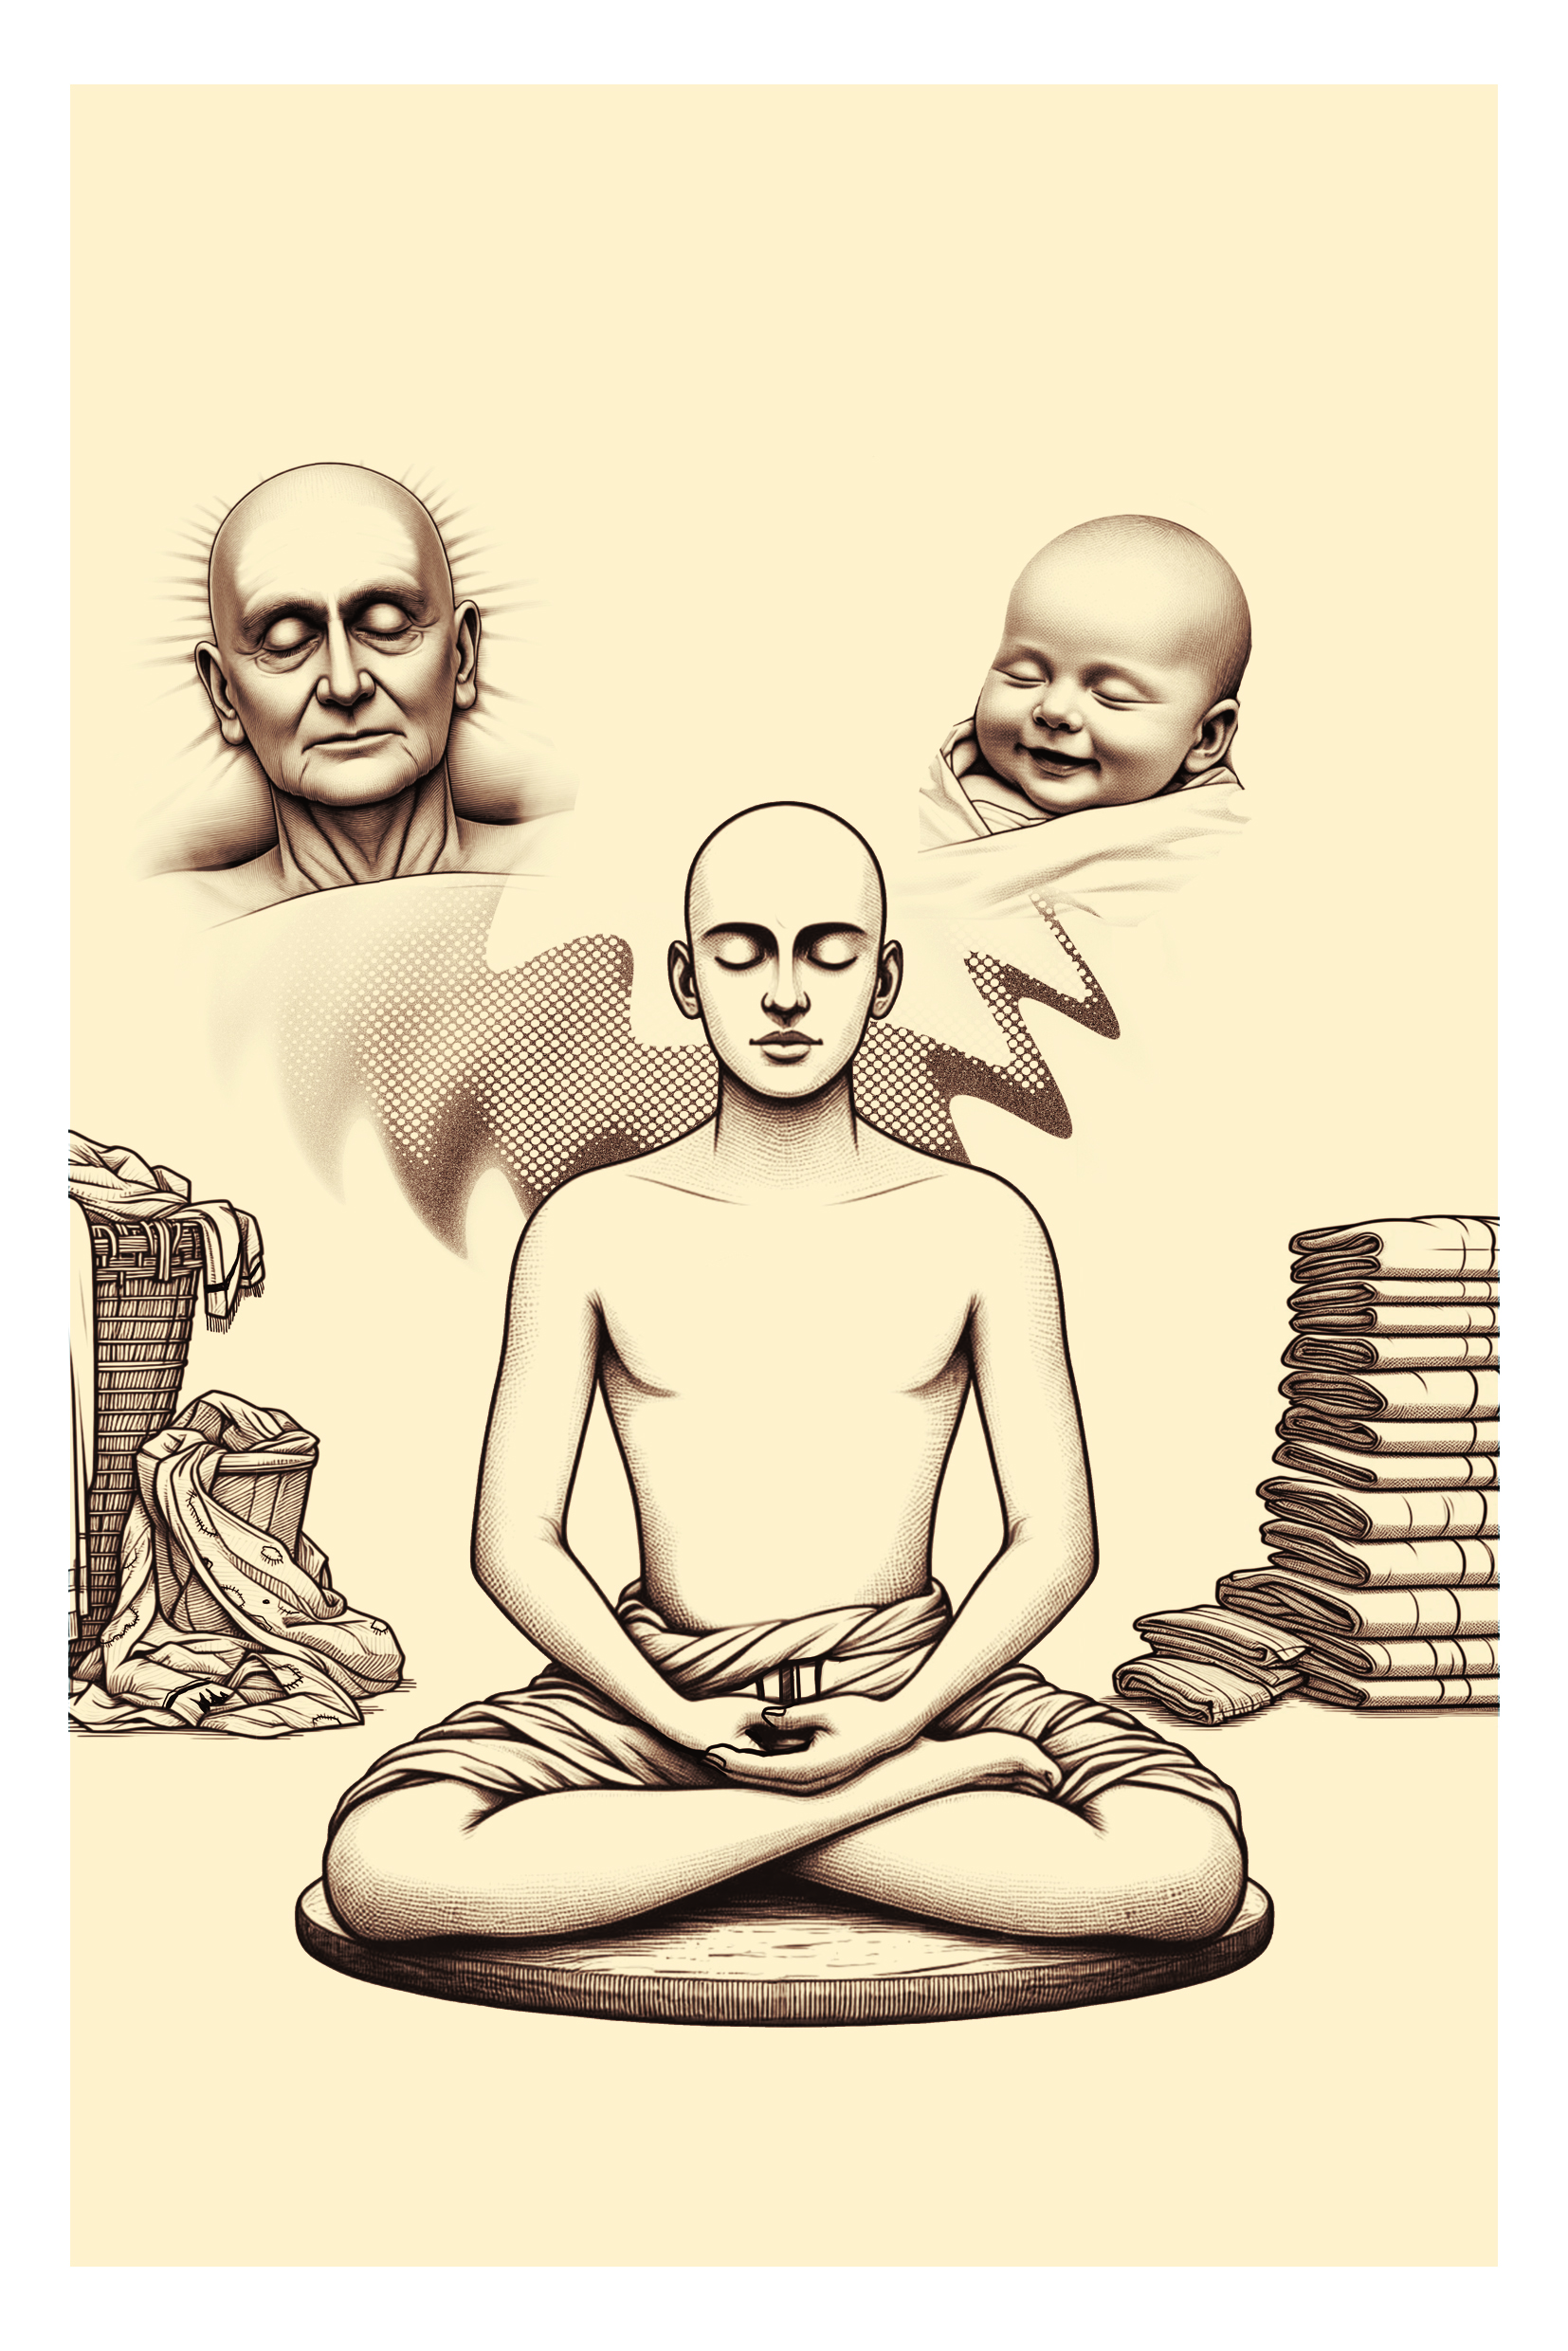
\includegraphics[width=\paperwidth, height=\paperheight, keepaspectratio]{./images/002.jpg}
\end{figure}
\restoregeometry % Restore original geometry settings
\newpage

\begin{mananam}{\mananamfont{ಮನನ ಶ್ಲೋಕ - ೨೩, ೨೪}}
\small \mananatext ನನ್ನ ಬಗ್ಗೆ ನನಗಿರುವ ದೃಷ್ಟಿಕೋನದಂತೆಯೇ ನನ್ನ ನಡವಳಿಕೆ, ಮನೋಭಾವ, ಜೀವನ ಮತ್ತು ಜೀವನದಾಚೆಗೂ  ಇರುತ್ತದೆ. ಸವಾಲುಗಳು, ತೊಂದರೆಗಳು, ನೋವು ಮತ್ತು ಅಂತಿಮವಾಗಿ ಸಾವಿನ ಭಯದಿಂದ ಜೀವನದ ಸನ್ನಿವೇಶಗಳನ್ನು ಎದುರಿಸಲು ನಾನು ಹೆದರುತ್ತೇನೆಯೇ? ಅಥವಾ, ಇದಕ್ಕೆ ವಿಪರೀತವಾಗಿ ನನ್ನ, ಮತ್ತು ಇತರರ ಬಗ್ಗೆ ನನಗೆ ಅಚಲವಾದ ದೂರದೃಷ್ಟಿ ಇದೆಯೇ?  ನನ್ನನ್ನು ನಾನು, ‘ಈ ದೇಹ, ಬುದ್ಧಿಯ ಪರಿಧಿಯೊಳಗೆ ಸೀಮಿತನಾದವನು’ ಎಂದು ಗುರುತಿಸಿಕೊಳ್ಳುತ್ತೇನೆಯೇ? 
\end{mananam}
\WritingHand\enspace\textbf{ಆತ್ಮ ವಿಮರ್ಶೆ}
\begin{inspiration}{\mananamfont ಸ್ಪೂರ್ತಿ}
\small \mananatext ಸ್ಥೂಲ ವಸ್ತುಗಳು, ಸ್ಥೂಲ ಅಂಶಗಳ ಮೇಲೆ ಮಾತ್ರ ಪರಿಣಾಮ ಬೀರಬಹುದು ಆದರೆ, ಸೂಕ್ಷ್ಮಅಂಶಗಳಿಗಲ್ಲ. ಹಾದು ಹೋಗುವ ಗಾಳಿ ಅಥವಾ ಬೆಂಕಿಯು ಆಕಾಶದ ಮೇಲೆ ಯಾವುದೇ ಪರಿಣಾಮ ಬೀರುವುದಿಲ್ಲ. ದೈಹಿಕ ಅಥವಾ ಮಾನಸಿಕ ರೂಪಾಂತರಗಳಿಂದ ಆತ್ಮಕ್ಕೆ ಏನೂ ಪರಿಣಾಮವಾಗುವುದಿಲ್ಲ.
\end{inspiration}
\newpage

\begin{mananam}{\mananamfont ಮನನ ಶ್ಲೋಕ - ೨೭}
\small \mananatext ಹೆಚ್ಚುತ್ತಿರುವ ವಯಸ್ಸು ಹಾಗೂ ವೃದ್ಧಾಪ್ಯ  ನನಗೆ ಭಯ ಉಂಟು ಮಾಡುತ್ತಿದೆಯೇ? ಬದಲಾವಣೆಗಳು ನನಗೆ ಆತಂಕ ಉಂಟುಮಾಡುತ್ತವೆಯೇ? ಜೀವನದ ಬದಲಾವಣೆಗಳನ್ನು ನಾನು ಶಾಂತ ರೀತಿಯಿಂದ ಸ್ವೀಕರಿಸಬಲ್ಲೆನೇ? ಬದಲಾಗುತ್ತಿರುವ ಈ ದೇಹದ ಲಕ್ಷಣ ಮತ್ತು ಸುತ್ತಲಿನ ಪರಿಸರದ ಬದಲಾವಣೆಗಳಿಗೆ ನಾನು ಸ್ವೀಕಾರ ಮನೋಭಾವದ ನಿಲುವನ್ನು ತಳೆಯಬಹುದೇ?
\end{mananam}
\WritingHand\enspace\textbf{ಆತ್ಮ ವಿಮರ್ಶೆ}
\begin{inspiration}{\mananamfont ಸ್ಪೂರ್ತಿ}
\small \mananatext  “ಕಾಲಾನಂತರದಲ್ಲಿ ಇದೂ ಕೂಡ ಹಾದು ಹೋಗುವುದು”  ಎಂದು ಒಂದು ಪುರಾತನ ಗಾದೆ ಇದೆ. ಈ ಗಾದೆಯ ಅರ್ಥವನ್ನು ಮನನ ಮಾಡಿ, ಅಂಗೀಕರಿಸುವುದರಿಂದ,  ಒಳ್ಳೆಯ ಸಮಯಗಳಲ್ಲಾಗಲೀ ಅಥವಾ ಕಷ್ಟದ ಸಮಯಗಳಲ್ಲಾಗಲೀ, ನಮ್ಮಲ್ಲಿ, ಎಲ್ಲವನ್ನೂ ( ಕಷ್ಟ, ಸುಖ ಇತ್ಯಾದಿ.,) ಸ್ವೀಕರಿಸುವ ಮನೋಭಾವ ಮತ್ತು  ‘ಕಡೆಗೆ ಎಲ್ಲವೂ ಒಳ್ಳೆಯದೇ  ಆಗುವುದು’ ಎಂಬ ನೆಮ್ಮದಿಯ ಮನೋಭಾವ ಉಂಟಾಗುವುದು. ವಿಶೇಷವಾಗಿ, ಕಷ್ಟದ ಸಮಯದಲ್ಲಿ ತಾಳ್ಮೆಯಿಂದ, ನಿಪುಣತೆಯಿಂದ ವರ್ತಿಸುವುದೇ ಒಂದು ಕಲೆ!
\end{inspiration}
\newpage

\slcol{\Index{ಆಶ್ಚರ್ಯವತ್ಪಶ್ಯತಿ ಕಶ್ಚಿದೇನ}ಮಾಶ್ಚರ್ಯ-\\ವದ್ವದತಿ ತಥೈವ ಚಾನ್ಯಃ ।\\
ಆಶ್ಚರ್ಯವಚ್ಚೈನಮನ್ಯಃ ಶೃಣೋತಿ \\ಶ್ರುತ್ವಾಪ್ಯೇನಂ ವೇದ ನ ಚೈವ ಕಶ್ಚಿತ್ ॥ ೨೯ ॥}
\cquote{ಈ ಆತ್ಮನನ್ನು ಒಬ್ಬಾನೊಬ್ಬನು ಆಶ್ಚರ್ಯವಾಗಿ ನೋಡುತ್ತಾನೆ. ಮತ್ತೊಬ್ಬನು ಆಶ್ಚರ್ಯವಾಗಿ ಹೇಳುತ್ತಾನೆ. ಮತ್ತೊಬ್ಬನು ಆಶ್ಚರ್ಯವಾಗಿ ಕೇಳುತ್ತಾನೆ. ಕೇಳಿದರೂ ಈ ಆತ್ಮನನ್ನು ಯಾರೂ ತಿಳಿಯಲಾರರು.\\}
\slcol{\Index{ದೇಹೀ ನಿತ್ಯಮವಧ್ಯೋऽಯಂ} ದೇಹೇ ಸರ್ವಸ್ಯ ಭಾರತ ।\\
ತಸ್ಮಾತ್ಸರ್ವಾಣಿ ಭೂತಾನಿ ನ ತ್ವಂ ಶೋಚಿತುಮರ್ಹಸಿ ॥ ೩೦ ॥}
\cquote{ಅರ್ಜುನ, ಎಲ್ಲರ ದೇಹದಲ್ಲಿರುವ ಈ ಆತ್ಮ ತತ್ವ ಕೊಲ್ಲಬರುವಂಥ ವಸ್ತುವಲ್ಲ. ಆದ್ದರಿಂದ ಯಾವ ಪ್ರಾಣಿಯ ಬಗೆಗೂ ನೀನು ವ್ಯಥೆಪಡುವ ಕಾರಣವಿಲ್ಲ.\\}
\slcol{\Index{ಸ್ವಧರ್ಮಮಪಿ ಚಾವೇಕ್ಷ್ಯ} ನ ವಿಕಂಪಿತುಮರ್ಹಸಿ ।\\
ಧರ್ಮ್ಯಾದ್ಧಿ ಯುದ್ಧಾಚ್ಛ್ರೇಯೋऽನ್ಯತ್ಕ್ಷತ್ರಿಯಸ್ಯ ನ ವಿದ್ಯತೇ ॥ ೩೧ ॥}
\cquote{ಯುದ್ಧವು ನಿನ್ನ ಸಹಜ ಧರ್ಮವೆಂಬುದನ್ನು ನೋಡಿಯಾದರೂ ನೀನು ಕಂಗೆಡಬಾರದು. ಕ್ಷತ್ರಿಯನಿಗೆ ಧರ್ಮಯುದ್ಧಕ್ಕಿಂತ ಬೇರೆ ಶ್ರೇಯಸ್ ಇಲ್ಲ.\\}
\slcol{\Index{ಯದೃಚ್ಛಯಾ ಚೋಪಪನ್ನಂ} ಸ್ವರ್ಗದ್ವಾರಮಪಾವೃತಮ್ ।\\
ಸುಖಿನಃ ಕ್ಷತ್ರಿಯಾಃ ಪಾರ್ಥ ಲಭಂತೇ ಯುದ್ಧಮೀದೃಶಮ್ ॥ ೩೨ ॥}
\cquote{ಅರ್ಜುನ, ತಾನಾಗಿ ಒದಗಿ ಬಂದ ಇಂತಹ ಯುದ್ಧವೆಂದರೆ ತೆರೆದಿಟ್ಟ ಸ್ವರ್ಗದ ಬಾಗಿಲು. ಇಂಥ ಯುದ್ಧವನ್ನು ಪುಣ್ಯಶಾಲಿಗಳಾದ ಕ್ಷತ್ರಿಯರು ಪಡೆಯುತ್ತಾರೆ.\\}
\slcol{\Index{ಅಥ ಚೇತ್ತ್ವಮಿಮಂ ಧರ್ಮ್ಯಂ} ಸಂಗ್ರಾಮಂ ನ ಕರಿಷ್ಯಸಿ ।\\
ತತಃ ಸ್ವಧರ್ಮಂ ಕೀರ್ತಿಂ ಚ ಹಿತ್ವಾ ಪಾಪಮವಾಪ್ಸ್ಯಸಿ ॥ ೩೩ ॥}
\cquote{ನೀನು ಈ ಧರ್ಮ ಯುದ್ಧವನ್ನು ಮಾಡದೆ ಬಿಟ್ಟರೆ ಸ್ವಧರ್ಮಭ್ರಷ್ಟನೂ ಕೀರ್ತಿಭ್ರಷ್ಟನೂ ಆಗಿ ಪಾಪಕ್ಕೆ ಗುರಿಯಾಗುವೆ.\\}
\slcol{\Index{ಅಕೀರ್ತಿಂ ಚಾಪಿ ಭೂತಾನಿ} ಕಥಯಿಷ್ಯಂತಿ ತೇऽವ್ಯಯಾಮ್ ।\\
ಸಂಭಾವಿತಸ್ಯ ಚಾಕೀರ್ತಿರ್ಮರಣಾದತಿರಿಚ್ಯತೇ ॥ ೩೪ ॥}
\cquote{ನಿನ್ನ ಅಪಕೀರ್ತಿಯನ್ನು ಜನರು ಅನಂತಕಾಲದವರೆಗೆ ಆಡಿಕೊಳ್ಳುತ್ತಾರೆ. ಮರ್ಯಾದಸ್ತನಿಗೆ ಅಪನಿಂದನೆಯು ಮರಣಕ್ಕಿಂತ ಕೀಳಾದದ್ದು.\\}
\slcol{\Index{ಭಯಾದ್ರಣಾದುಪರತಂ} ಮಂಸ್ಯಂತೇ ತ್ವಾಂ ಮಹಾರಥಾಃ ।\\
ಯೇಷಾಂ ಚ ತ್ವಂ ಬಹುಮತೋ ಭೂತ್ವಾ ಯಾಸ್ಯಸಿ ಲಾಘವಮ್ ॥ ೩೫ ॥}
\cquote{ನಿನ್ನನ್ನು, ಭಯದಿಂದ ಯುದ್ಧವನ್ನು ಬಿಟ್ಟವನೆಂದು ಈ ಕ್ಷತ್ರಿಯ ವೀರರು ತಿಳಿಯುತ್ತಾರೆ. ಇಲ್ಲಿಯವರೆಗೆ ನಿನ್ನನ್ನು ಗೌರವದಿಂದ ನೋಡಿದವರೇ ಈಗ ಹಗುರಾಗಿ ನೋಡುವರು.}

\begin{mananam}{\mananamfont ಮನನ ಶ್ಲೋಕ - ೨೯}
\small \mananatext ನಾನು ನನ್ನ ಜೀವನವನ್ನು ನಿತ್ಯವೂ ನವೀನ ದೃಷ್ಟಿಕೋನದಿಂದ ನೋಡುತ್ತೇನೆಯೇ ಹಾಗೂ ಲವಲವಿಕೆಯಿಂದ ಈ ಜೀವನವನ್ನು ಆಲಂಗಿಸುತ್ತೇನೆಯೇ? ನಾನು ಪಕ್ಷಪಾತಿಯಾಗಿದ್ದೀನೆಯೇ? ಎಲ್ಲದರ ಬಗ್ಗೆ ವಿಮರ್ಶಾತ್ಮಕ ಹಾಗೂ ತೀವ್ರವಾದ (ಅಂದರೆ, ಇದು ಹೀಗೇ ಸರಿ, ಇದಾದರೆ ತಪ್ಪು ಎಂದು, ಎಲ್ಲಾ ಅನಾವಶ್ಯಕವಾದ ಹಾಗೂ ಮುಖ್ಯವಲ್ಲದ ಪ್ರಾಪಂಚಿಕ ವಿಷಯಗಳಲ್ಲೂ ಕೂಡ ) ನಿರ್ಣಯ ತೆಗೆದುಕೊಳ್ಳುತ್ತೇನೆಯೇ? ನನ್ನ ಈ ಕ್ಷಣದ ಅನುಭವಕ್ಕೂ( ನವೀನ ಅನುಭವ ), ಹಳೆಯ  ಅನುಭವದ ಮೂಟೆಯಿಂದ ಆಧರಿಸಿದ ವಿಮರ್ಶಾತ್ಮಕ ಬಣ್ಣವನ್ನೇ ಬಳೆಯುತ್ತೇನೆಯೇ?
\end{mananam}
\WritingHand\enspace\textbf{ಆತ್ಮ ವಿಮರ್ಶೆ}
\begin{inspiration}{\mananamfont ಸ್ಪೂರ್ತಿ}
\small \mananatext ಮಗು ಎಲ್ಲವನ್ನೂ ಆಶ್ಚರ್ಯ ಮತ್ತು ಕುತೂಹಲದಿಂದ ನೋಡುತ್ತದೆ. ಅದು ಎಲ್ಲವನ್ನೂ ಹೊಸತನ ಮತ್ತು ಸಂತೋಷದಿಂದ ಅನುಭವಿಸುತ್ತದೆ; ಏಕೆಂದರೆ ಅದರ ಮನದಲ್ಲಿ ಯಾವುದೇ ಕಟ್ಟುಪಾಡುಗಳೂ ಇರುವುದಿಲ್ಲ.ಆದರೆ ಅದು ಬೆಳೆದಂತೆ, ತಾನು ಏನನ್ನು ಮಾಡಬೇಕು, ಕೇಳಬೇಕು ಎಂದು ಬಯಸುವ ಕಡೆಗೆ ಪಕ್ಷಪಾತಭಾವನೆ ಬೆಳೆಯಿಸಿಕೊಳ್ಳುವುದು. ತಾನು ಬಯಸಿದ ಪ್ರಾಪಂಚಿಕ ಸುಖವು ಸಿಗದಿದ್ದಾಗ,  ಶೀಘ್ರದಲ್ಲಿಯೇ ಜೀವನವು ಬೇಸರ, ಮಂದ, ನಿರಾಶಾದಾಯಕವಾಗುತ್ತದೆ; ನಿಮ್ಮೊಳಗಿನ ಮಗುವನ್ನು ಪುನರ್ಜೀವಗೊಳಿಸಿ. ಜೀವನದ ಪ್ರತಿ ಕ್ಷಣವನ್ನೂ ಹಾಗೂ ಇತರರ ಜೊತೆಗಿನ ಸಂಬಂಧಗಳನ್ನೂ, ತಾಜಾತನ ಮತ್ತು ನಿಷ್ಕಲ್ಮಶ ಮನಸ್ಸಿನಿಂದ ಅನುಭವಿಸಿ. ಹಾಗಾದಾಗ, ಈ ಜೀವನ, ಬೇಸರವಾದ ಏಕತಾನತೆ ಎನಿಸದೆ, ಜೀವನದಲ್ಲಿ ಹುಮ್ಮಸ್ಸು ತಂತಾನೇ ಚಿಮ್ಮುತ್ತದೆ!
\end{inspiration}
\newpage

\begin{mananam}{\mananamfont ಮನನ ಶ್ಲೋಕ - ೩೧}
\small \mananatext ನನ್ನ ಜೀವನದಲ್ಲಿ ಅನ್ಯಾಯವಾಗಿ ನನ್ನ ಮೇಲೆ ಕೆಲವು ಕರ್ತವ್ಯಗಳನ್ನು ಹೇರಲಾಗಿದೆ ಎಂದು ಭಾವಿಸುತ್ತೇನೆಯೇ? ಆದರೆ, ಈ ಕರ್ತವ್ಯಗಳನ್ನು ನಿಭಾಯಿಸಲು ಕಲಿತರೆ ನನ್ನ ಜೀವನ ಪ್ರಕಾಶಮಯ ಹಾಗೂ ಲಾಭದಾಯಕವಾಗಬಹುದೇ? ನನ್ನ ಜೀವನದಲ್ಲಿ ಬರುವ ಕರ್ತವ್ಯಗಳನ್ನು ಗೊಣಗದೆ,ದೂರದೆ, ಸಂಪೂರ್ಣ ಸ್ವೀಕಾರ ಮನೋಭಾವದಿಂದ ಮಾಡಲು ಕಲಿತರೆ ಒಳ್ಳೆಯದಲ್ಲವೇ? ಹಾಗೂ, ಸ್ವಇಚ್ಛೆಯಿಂದ ಮಾಡುವ ಕೆಲಸದಿಂದ ಉತ್ಸಾಹವಿರುತ್ತದೆ, ಹೃದಯ ಹಗುರವಾಗುತ್ತದೆ; ಸ್ವಇಚ್ಛೆ ಇಲ್ಲದಿದ್ದಲ್ಲಿ, ಕೆಲಸ ಪ್ರಾರಂಭಿಸುವ  ಮೊದಲೇ ಶರೀರದಲ್ಲಿ ಆಯಾಸ ಹಾಗೂ ಚಡಪಡಿಕೆ ಅನುಭವಿಸುತ್ತೇವೆ. 
\end{mananam}
\WritingHand\enspace\textbf{ಆತ್ಮ ವಿಮರ್ಶೆ}
\begin{inspiration}{\mananamfont ಸ್ಪೂರ್ತಿ}
\small \mananatext ನಮಗೆ ಇಷ್ಟವಾಗದ ಕರ್ತವ್ಯಗಳು ಎಂದು ಬಾಹ್ಯಕ್ಕೆ ತೋರಿದರೂ ಕೂಡ ಅವುಗಳು,  ನಮ್ಮನ್ನು ಕೆಲವು ಅವಕಾಶಗಳು ಮತ್ತು ಕೌಶಲಗಳೊಂದಿಗೆ ಸಜ್ಜುಗೊಳಿಸುತ್ತವೆ. ಪ್ರಕೃತಿಯ ನಿಯಮವೆಂದರೆ, ಭವ್ಯವಾದ ಕಾಲದ ಮಾನದಂಡದಲ್ಲಿ,  ಎಂದಿಗೂ, ಯಾರಿಗೂ ಅನ್ಯಾಯವಾಗುವುದಿಲ್ಲ ಮತ್ತು ನಮ್ಮ ಯಾವುದೇ ಪ್ರಯತ್ನಕ್ಕೂ ಪ್ರತಿಫಲ ದೊರಕದೇ ಇರುವುದಿಲ್ಲ.
\end{inspiration}
\newpage

\begin{mananam}{\mananamfont ಮನನ ಶ್ಲೋಕ - ೩೩}
\small \mananatext ನನ್ನ ಇಂದಿನ ಪರಿಸ್ಥಿತಿಯಲ್ಲಿ ನನ್ನ ಧರ್ಮ ಯಾವುದು (ಅಂದರೆ, ನಾಲಕ್ಕು ಆಶ್ರಮಗಳು ಹಾಗೂ ಜೀವನದ ಕರ್ತವ್ಯದ ಆಧಾರದಮೇಲೆ ನಿಂತಿರುವ ಧರ್ಮ ) ಕಾಲಕ್ಕೆ ತಕ್ಕಂತೆ ನಾನು ನನ್ನ ಧರ್ಮವನ್ನು ಹೇಗೆ ಪರಿಪಾಲಿಸುತ್ತೇನೆ? ಆತ್ಮ ಸಮ್ಮಾನ ಹಾಗೂ ನನ್ನ ಗೌರವ ಕಾಪಾಡಿಕೊಳ್ಳಲು, ನಾನು ಹೇಗೆ ವರ್ತಿಸಬೇಕು? ನಾನು, ನನ್ನ ಕರ್ತವ್ಯ ಅಥವಾ ಜೀವನದ ಮೌಲ್ಯಗಳನ್ನು ಬೆಂಬಲಿಸುವ ಬದಲಾಗಿ, ಅವುಗಳಿಂದ ವಿಮುಖನಾಗಿದ್ದೇಯೇ? ಅವುಗಳನ್ನು ತೊರೆಯುತ್ತಿದ್ದೇನೆಯೇ? ನನ್ನ ಜೀವನದ ಸಂಘರ್ಷಗಳನ್ನು ಎದುರಿಸಲು ಹಾಗೂ, ನನ್ನ ಧರ್ಮ ನೆರವೇರಿಸಲು, ನಾನು ಹೆದರುತ್ತೇನೆಯೇ?
\end{mananam}
\WritingHand\enspace\textbf{ಆತ್ಮ ವಿಮರ್ಶೆ}
\begin{inspiration}{\mananamfont ಸ್ಪೂರ್ತಿ}
\small \mananatext ಪರಮಸತ್ಯವನ್ನು ಪಡೆಯಲು, ಪೂರ್ಣ ಹೃದಯದಿಂದ, ಶ್ರದ್ಧೆಯಿಂದ ಬದ್ಧನಾಗಿರುವವನು, ತ್ಯಾಗ ಮಾಡಿದಾಗ ಮಾತ್ರವೇ ಸ್ವೀಕಾರಾರ್ಹವಾಗುವುದು. ಒಬ್ಬನು, ತನ್ನ ರಾಷ್ಟ್ರಕ್ಕೋಸ್ಕರ ಅಥವಾ, ಒಂದು ದೊಡ್ಡ ಸಮುದಾಯಕೋಸ್ಕರ ಸೇವೆ ಸಲ್ಲಿಸುವುದರಲ್ಲಿ ನಿರತನಾಗಿದ್ದರೆ, ಹಾಗೂ ಆತನು, ಇದರಿಂದಾಗಿ ತನ್ನ ಕುಟುಂಬದ ಜವಾಬ್ದಾರಿಯನ್ನು ಹೊರಲು ವಿಫಲನಾದಲ್ಲಿ, ಇದು ( ತ್ಯಾಗ) ಸ್ವೀಕಾರಾರ್ಹವಾಗಿದೆ; ಅಂಥವನು ಕ್ಷಮಾರ್ಹನು. ಆದರೆ, ಸೋಮಾರಿತನ ಹಾಗೂ ಸ್ವಾರ್ಥದ ಆಕಾಂಕ್ಷೆಗಳ ಬೆನ್ನಟ್ಟಿ, ತನ್ನ ಕುಟುಂಬದ ಹಾಗೂ ಸಮಾಜದ ಬಗ್ಗೆ ತೋರಬೇಕಾದ ಕರ್ತವ್ಯ  ಮತ್ತು ಜವಾಬ್ದಾರಿಯಿಂದ ವಿಮುಖನಾದಲ್ಲಿ, ಅಂಥವನನ್ನು ನಕರಾತ್ಮಕತೆ ಮತ್ತು ಭಯಗಳು ಕಾಡುತ್ತವೆ; ಇಂಥಹ ತಪ್ಪು ಭಾವನೆಗಳಿಗೆ ಎಡೆ ಕೊಡುವುದು, ತನ್ನ ಆತ್ಮಕ್ಕೂ ಹಾಗೂ, ಇತರರಿಗೂ ಮಾಡುವ ಅತ್ಯಧಿಕ ಅಪರಾಧವೆಂದು ಪರಿಗಣಿಸಲ್ಪಡುತ್ತದೆ. 
\end{inspiration}
\newpage


\slcol{\Index{ಅವಾಚ್ಯವಾದಾಂಶ್ಚ ಬಹೂನ್ವ}ದಿಷ್ಯಂತಿ ತವಾಹಿತಾಃ ।\\
ನಿಂದಂತಸ್ತವ ಸಾಮರ್ಥ್ಯಂ ತತೋ ದುಃಖತರಂ ನು ಕಿಮ್ ॥ ೩೬ ॥}
\cquote{ಶತ್ರುಗಳು ನಿನ್ನ ಪರಾಕ್ರಮವನ್ನು ನಿಂದಿಸಿ ಮಾತನಾಡುವರು. ಇದಕ್ಕಿಂತ ಹೆಚ್ಚಿನ ದುಃಖ ಯಾವುದು?\\}
\slcol{\Index{ಹತೋ ವಾ ಪ್ರಾಪ್ಸ್ಯಸಿ} ಸ್ವರ್ಗಂ ಜಿತ್ವಾ ವಾ ಭೋಕ್ಷ್ಯಸೇ ಮಹೀಮ್ ।\\
ತಸ್ಮಾದುತ್ತಿಷ್ಠ ಕೌಂತೇಯ ಯುದ್ಧಾಯ ಕೃತನಿಶ್ಚಯಃ ॥ ೩೭ ॥}
\cquote{ಸತ್ತರೆ ಸ್ವರ್ಗವನ್ನು ಸೇರುವೆ, ಗೆದ್ದರೆ ಭೂಮಿಯನ್ನು ಆಳುವೆ. ಆದ್ದರಿಂದ ಅರ್ಜುನ ಕಾದುವುದಕ್ಕೆ ಮನಸ್ಸು ಗಟ್ಟಿಮಾಡಿಕೊಂಡು ಏಳು.\\}
\slcol{\Index{ಸುಖದುಃಖೇ ಸಮೇ ಕೃತ್ವಾ} ಲಾಭಾಲಾಭೌ ಜಯಾಜಯೌ ।\\
ತತೋ ಯುದ್ಧಾಯ ಯುಜ್ಯಸ್ವ ನೈವಂ ಪಾಪಮವಾಪ್ಸ್ಯಸಿ ॥ ೩೮ ॥}
\cquote{ಸುಖದುಃಖಗಳನ್ನು, ಲಾಭನಷ್ಟಗಳನ್ನು, ಜಯಾಪಜಯಗಳನ್ನು ಸಮಾನವಾಗಿ ತಿಳಿದು ಯುದ್ಧವನ್ನು ಮಾಡು. ಹಾಗಾದರೆ ಪಾಪಗಳು ನಿನ್ನನ್ನು ಅಂಟಲಾರವು.\\}
\slcol{\Index{ಏಷಾ ತೇऽಭಿಹಿತಾ ಸಾಂಖ್ಯೇ} ಬುದ್ಧಿರ್ಯೋಗೇ ತ್ವಿಮಾಂ ಶೃಣು ।\\
ಬುದ್ಧ್ಯಾ ಯುಕ್ತೋ ಯಯಾ ಪಾರ್ಥ ಕರ್ಮಬಂಧಂ ಪ್ರಹಾಸ್ಯಸಿ ॥ ೩೯ ॥}
\cquote{ಪಾರ್ಥಾ, ಆತ್ಮನ ವಿಚಾರವಾಗಿ ಈ ತಿಳುವಳಿಕೆಯನ್ನು ನಿನಗೆ ಹೇಳಿದ್ದಾಯಿತು. ಇಲ್ಲಿಯವರೆಗೆ ಸಾಂಖ್ಯ ಜ್ಞಾನವನ್ನು ಬೋಧಿಸಿದೆನು. ಯಾವ ಜ್ಞಾನವನ್ನು ಹೊಂದಿದರೆ ಕರ್ಮಬಂಧಕ್ಕೆ ಸಿಗುವುದಿಲ್ಲವೋ, ಆ ಯೋಗಸಂಬಂಧವಾದ ಜ್ಞಾನವನ್ನು ಇನ್ನು ಹೇಳುತ್ತೇನೆ ಕೇಳು.\\}
\slcol{\Index{ನೇಹಾಭಿಕ್ರಮನಾಶೋऽಸ್ತಿ} ಪ್ರತ್ಯವಾಯೋ ನ ವಿದ್ಯತೇ ।\\
ಸ್ವಲ್ಪಮಪ್ಯಸ್ಯ ಧರ್ಮಸ್ಯ ತ್ರಾಯತೇ ಮಹತೋ ಭಯಾತ್ ॥ ೪೦ ॥}
\cquote{ಇದರ ಆರಂಭ ಮಾತ್ರವೂ ವ್ಯರ್ಥವಲ್ಲ. ಇದರಲ್ಲಿ ದೋಷ ಉಂಟಾಗುವುದಿಲ್ಲ. ಈ ಧರ್ಮದ ಅಲ್ಪಾಚರಣೆ ಕೂಡ ಹಿರಿಯ ಪಾತಕದಿಂದ ಪಾರು ಮಾಡುತ್ತದೆ.\\}
\slcol{\Index{ವ್ಯವಸಾಯಾತ್ಮಿಕಾ ಬುದ್ಧಿ}ರೇಕೇಹ ಕುರುನಂದನ ।\\
ಬಹುಶಾಖಾ ಹ್ಯನಂತಾಶ್ಚ ಬುದ್ಧಯೋऽವ್ಯವಸಾಯಿನಾಮ್ ॥ ೪೧ ॥}
\cquote{ಅರ್ಜುನ, ಈ ಸಾಧನಗಳಲ್ಲಿ ನೆಲೆಗೆ ನಿಂತ ಬುದ್ಧಿಯು ಒಂದೇ ಮುಖವಾಗಿರುವುದು. ನೆಲೆಗೆ ನಿಲ್ಲದವರ ಬುದ್ಧಿಯು ಅನೇಕ ಕೊಂಬೆಗಳುಳ್ಳದ್ದಾಗಿ ಬಗೆ ಬಗೆಯಾಗಿರುವುದು. \\}
\slcol{\Index{ಯಾಮಿಮಾಂ ಪುಷ್ಪಿತಾಂ} ವಾಚಂ ಪ್ರವದಂತ್ಯವಿಪಶ್ಚಿತಃ ।\\
ವೇದವಾದರತಾಃ ಪಾರ್ಥ ನಾನ್ಯದಸ್ತೀತಿ ವಾದಿನಃ ॥ ೪೨ ॥}
\cquote{ಅರ್ಜುನ, ದಡ್ಡರು ವೇದದ ಮೇಲ್ನೋಟಕ್ಕೆ ಕಾಣುವ ಹೂವಿನಂತ ಮಾತಿಗೆ ಮರುಳಾಗುತ್ತಾರೆ. ಅದರ ಆಚೆಗಿರುವ ಭಗವತ್ತತ್ವವೆಂಬ ಹಣ್ಣು ಅವರಿಗೆ ಕಾಣಿಸದು. ಅದಕ್ಕೆಂದೇ ಅವರು ಅದನ್ನು ನಿರಾಕರಿಸಿಬಿಡುತ್ತಾರೆ.\\}

\newpage
\begin{mananam}{\mananamfont ಮನನ ಶ್ಲೋಕ - ೩೮}
\small \mananatext ಜೀವನದಲ್ಲಿ ನಾನು ಎದುರಿಸುವ ಯಾವುದೇ ಸವಾಲಿನ ಬಗ್ಗೆ ನನ್ನ ಮನೋಭಾವ ಏನು? ನಾನು ಯಾವುದೇ ತರಹದ ಫಲಿತಾಂಶದ ಕಡೆಗೆ ಸಮಚಿತ್ತನಾಗಿದ್ದೇನೆಯೇ? ನನ್ನ ಅತ್ಯುತ್ತಮ ಪ್ರಯತ್ನದ ಹೊರತಾಗಿಯೂ, ಒಳ್ಳೆಯ ಫಲಿತಾಂಶ ಬಂದಾಗ ಅದರ ಬಗ್ಗೆ ಮೋಹ ಮತ್ತು ಅಹಿತಕರ ಫಲಿತಾಂಶ ಬಂದಾಗ ಮಾನಸಿಕವಾಗಿ ವಿಮುಖತೆಯನ್ನು ಅನುಭವಿಸುತ್ತೇನೆಯೇ? ಗೆಲುವನ್ನು ಬಯಸದೇ, ಸೋಲನ್ನು ತಿರಸ್ಕರಿಸದೇ, ಲಾಭವನ್ನು ಹುಡುಕುವ ಮತ್ತು ನಷ್ಟವನ್ನು ತಪ್ಪಿಸುವ ಪ್ರೇರಣೆ ಇಲ್ಲದೇ, ಜೀವನದಲ್ಲಿ  ಕಾರ್ಯನಿರ್ವಹಿಸಲು ಕಲಿಯಬಹುದೇ?

\end{mananam}
\WritingHand\enspace\textbf{ಆತ್ಮ ವಿಮರ್ಶೆ}
\begin{inspiration}{\mananamfont ಸ್ಪೂರ್ತಿ}
\small \mananatext ಯಾವಾಗಲೂ ಗೆಲುವನ್ನು ಬಯಸುವುದು ಮತ್ತು ಸಂತೋಷವಾಗಿರಲು ಬಯಸುವುದು ಎಲ್ಲರಲ್ಲಿ ಸಹಜವಾಗಿರುವ ಒಲವು. ಹಾಗೆಯೇ ಅಹಿತಕರವಾದದ್ದನ್ನು ತಪ್ಪಿಸುವುದು ಮತ್ತು ಎಂದಿಗೂ ಸೋಲನ್ನು ಬಯಸದೇ ಇರುವುದೂ ಕೂಡ, ಸಹಜವಾದ ಪ್ರವೃತ್ತಿಯಾಗಿದೆ. ಆದರೆ, ನಿಜವಾದ ಸ್ವಾತಂತ್ರ್ಯ ಹೊಂದಿದ (ಅಂದರೆ, ಆತ್ಮಜ್ಞಾನಿಗೆ )ವ್ಯಕ್ತಿಗೆ,  ಎಲ್ಲಾ ಕ್ರಿಯೆಗಳೂ ನೀರಿನಲ್ಲಿ ರೇಖೆಗಳನ್ನು  ಎಳೆದಂತೆ; ಅವನು ಮಾನಸಿಕವಾಗಿ ಕಳಂಕರಹಿತ ಆದುದರಿಂದ, ಯಾವುದೇ ತರಹದ ಕರ್ಮದ ಬಂಧನ ಅವನಿಗಿಲ್ಲ.
\end{inspiration}
\newpage


\slcol{\Index{ಕಾಮಾತ್ಮಾನಃ ಸ್ವರ್ಗಪರಾ} ಜನ್ಮಕರ್ಮಫಲಪ್ರದಾಮ್ ।\\
ಕ್ರಿಯಾವಿಶೇಷಬಹುಲಾಂ ಭೋಗೈಶ್ವರ್ಯಗತಿಂ ಪ್ರತಿ ॥ ೪೩ ॥}
\cquote{ಅವರು ಬಯಕೆಯ ಬೆನ್ನು ಹತ್ತಿದವರು. ಸ್ವರ್ಗವೇ ಪುರುಷಾರ್ಥ ಎಂದು ಭ್ರಮಿಸಿದವರು. ನಮ್ಮನ್ನು ಹುಟ್ಟು ಸಾವುಗಳ ಸುಳಿಯಲ್ಲಿ ಸಿಕ್ಕಿಸುವ ಕರ್ಮಕಾಂಡದ ಕ್ಷಣಿಕ ಭೋಗಭಾಗ್ಯಗಳಿಗೆ ಮರುಳಾದವರು.\\}
\slcol{\Index{ಭೋಗೈಶ್ವರ್ಯಪ್ರಸಕ್ತಾನಾಂ} ತಯಾಪಹೃತಚೇತಸಾಮ್ ।\\
ವ್ಯವಸಾಯಾತ್ಮಿಕಾ ಬುದ್ಧಿಃ ಸಮಾಧೌ ನ ವಿಧೀಯತೇ ॥ ೪೪ ॥}
\cquote{ಇಂದ್ರಿಯ ಭೋಗ ಮತ್ತು ಸಂಪತ್ತುಗಳಲ್ಲಿ ಆಸಕ್ತರಾದ ಇಂಥವರು ಫಲಸ್ತುತಿಗಳ (ಹೊಗಳಿಕೆಯ) ಮಾತಿನ ಸೆಳೆತಕ್ಕೆ ಮರುಳಾಗುತ್ತಾರೆ. ಅಂತವರ ಮನಸ್ಸಿನಲ್ಲಿ ನೆಲೆ ನಿಂತ ತತ್ವದ ತಿಳುವಳಿಕೆ ಉಂಟಾಗುವುದಿಲ್ಲ.\\}
\slcol{\Index{ತ್ರೈಗುಣ್ಯವಿಷಯಾ ವೇದಾ} ನಿಸ್ತ್ರೈಗುಣ್ಯೋ ಭವಾರ್ಜುನ ।\\
ನಿರ್ದ್ವಂದ್ವೋ ನಿತ್ಯಸತ್ತ್ವಸ್ಥೋ ನಿರ್ಯೋಗಕ್ಷೇಮ ಆತ್ಮವಾನ್ ॥ ೪೫ ॥}
\cquote{ಅರ್ಜುನಾ, ವೇದಗಳು ತ್ರಿಗುಣ ರೂಪವಾದ ಸಂಸಾರವನ್ನು ಹೇಳುತ್ತವೆ. ನೀನು ತ್ರಿಗುಣಾತೀತನು ದ್ವಂದ್ವರಹಿತನು ಆಗು. ಶುದ್ಧ ಸತ್ವವನ್ನು ಆಶ್ರಯಿಸುವವನಾಗಿಯೂ ಯೋಗ ಕ್ಷೇಮಗಳ ಚಿಂತೆ ಇಲ್ಲದವನಾಗಿ  ಆಗು. ಆತ್ಮನಿಷ್ಟನಾಗಿರು.\\}
\slcol{\Index{ಯಾವಾನರ್ಥ ಉದಪಾನೇ} ಸರ್ವತಃ ಸಂಪ್ಲುತೋದಕೇ ।\\
ತಾವಾನ್ಸರ್ವೇಷು ವೇದೇಷು ಬ್ರಾಹ್ಮಣಸ್ಯ ವಿಜಾನತಃ ॥ ೪೬ ॥}
\cquote{ಬಾವಿಯಿಂದ ಆಗುವ ಪ್ರಯೋಜನ ಎಲ್ಲೆಡೆಯೂ ತುಂಬಿ ಹರಿಯುವ ಸಮುದ್ರದಿಂದ ಆಗಿಯೇ ಆಗುತ್ತದೆ. ಹಾಗೆಯೇ ವೇದದಲ್ಲಿ ಹೇಳಿರುವ ಎಲ್ಲಾ ಫಲಗಳು ಬ್ರಹ್ಮ ಜ್ಞಾನಿಗೆ ಸಿಕ್ಕೇ ಸಿಗುವುದು.\\}
\slcol{\Index{ಕರ್ಮಣ್ಯೇವಾಧಿಕಾರಸ್ತೇ ಮಾ} ಫಲೇಷು ಕದಾಚನ ।\\
ಮಾ ಕರ್ಮಫಲಹೇತುರ್ಭೂರ್ಮಾ ತೇ ಸಂಗೋऽಸ್ತ್ವಕರ್ಮಣಿ ॥ ೪೭ ॥}
\cquote{ಕರ್ಮ ಮಾಡುವುದಷ್ಟೇ ನಿನ್ನ ಹಕ್ಕು. ಕರ್ಮಫಲದ ಮೇಲೆ ಹಕ್ಕು ಸಾಧಿಸಬೇಡ. ಫಲದ ಆಸೆಯಿಂದ ಕರ್ಮ ಮಾಡಲು ಬೇಡ. ಹಾಗೆಯೇ ಕರ್ಮ ತ್ಯಾಗದ ಕಡೆಗೂ ನಿನ್ನ ಒಲವು ಹರಿಯದಿರಲಿ.\\}
\slcol{\Index{ಯೋಗಸ್ಥಃ ಕುರು ಕರ್ಮಾಣಿ} ಸಂಗಂ ತ್ಯಕ್ತ್ವಾ ಧನಂಜಯ ।\\
ಸಿದ\char"0CCD\char"0CA7\;\char"0CCD\char"0CAFಸಿ\char"0CA6\char"0CCD\char"0CA7\char"0CCB\;\char"0CCD\char"0CAFಃ  ಸಮೋ ಭೂತ್ವಾ ಸಮತ್ವಂ ಯೋಗ ಉಚ್ಯತೇ ॥ ೪೮ ॥}
\cquote{ಅರ್ಜುನ, ಯೋಗ ನಿಷ್ಠನಾಗಿ ಫಲಕ್ಕಾಗಿ ಆಸೆ ಮಾಡದೆ ಫಲ ದೊರೆತರೆ ಹಿಗ್ಗದೆ ಸಿಗದಿದ್ದರೆ ಕುಗ್ಗದೇ ಒಂದೇ ಭಾವದಿಂದ ಕರ್ಮವನ್ನು ಮಾಡು. ಈ ಸಮದೃಷ್ಟಿಯೇ ನಿಜವಾದ ಯೋಗ.\\}

\clearpage
\newgeometry{margin=0pt} % Apply margin only for this page
\thispagestyle{empty}
\begin{figure}
\centering
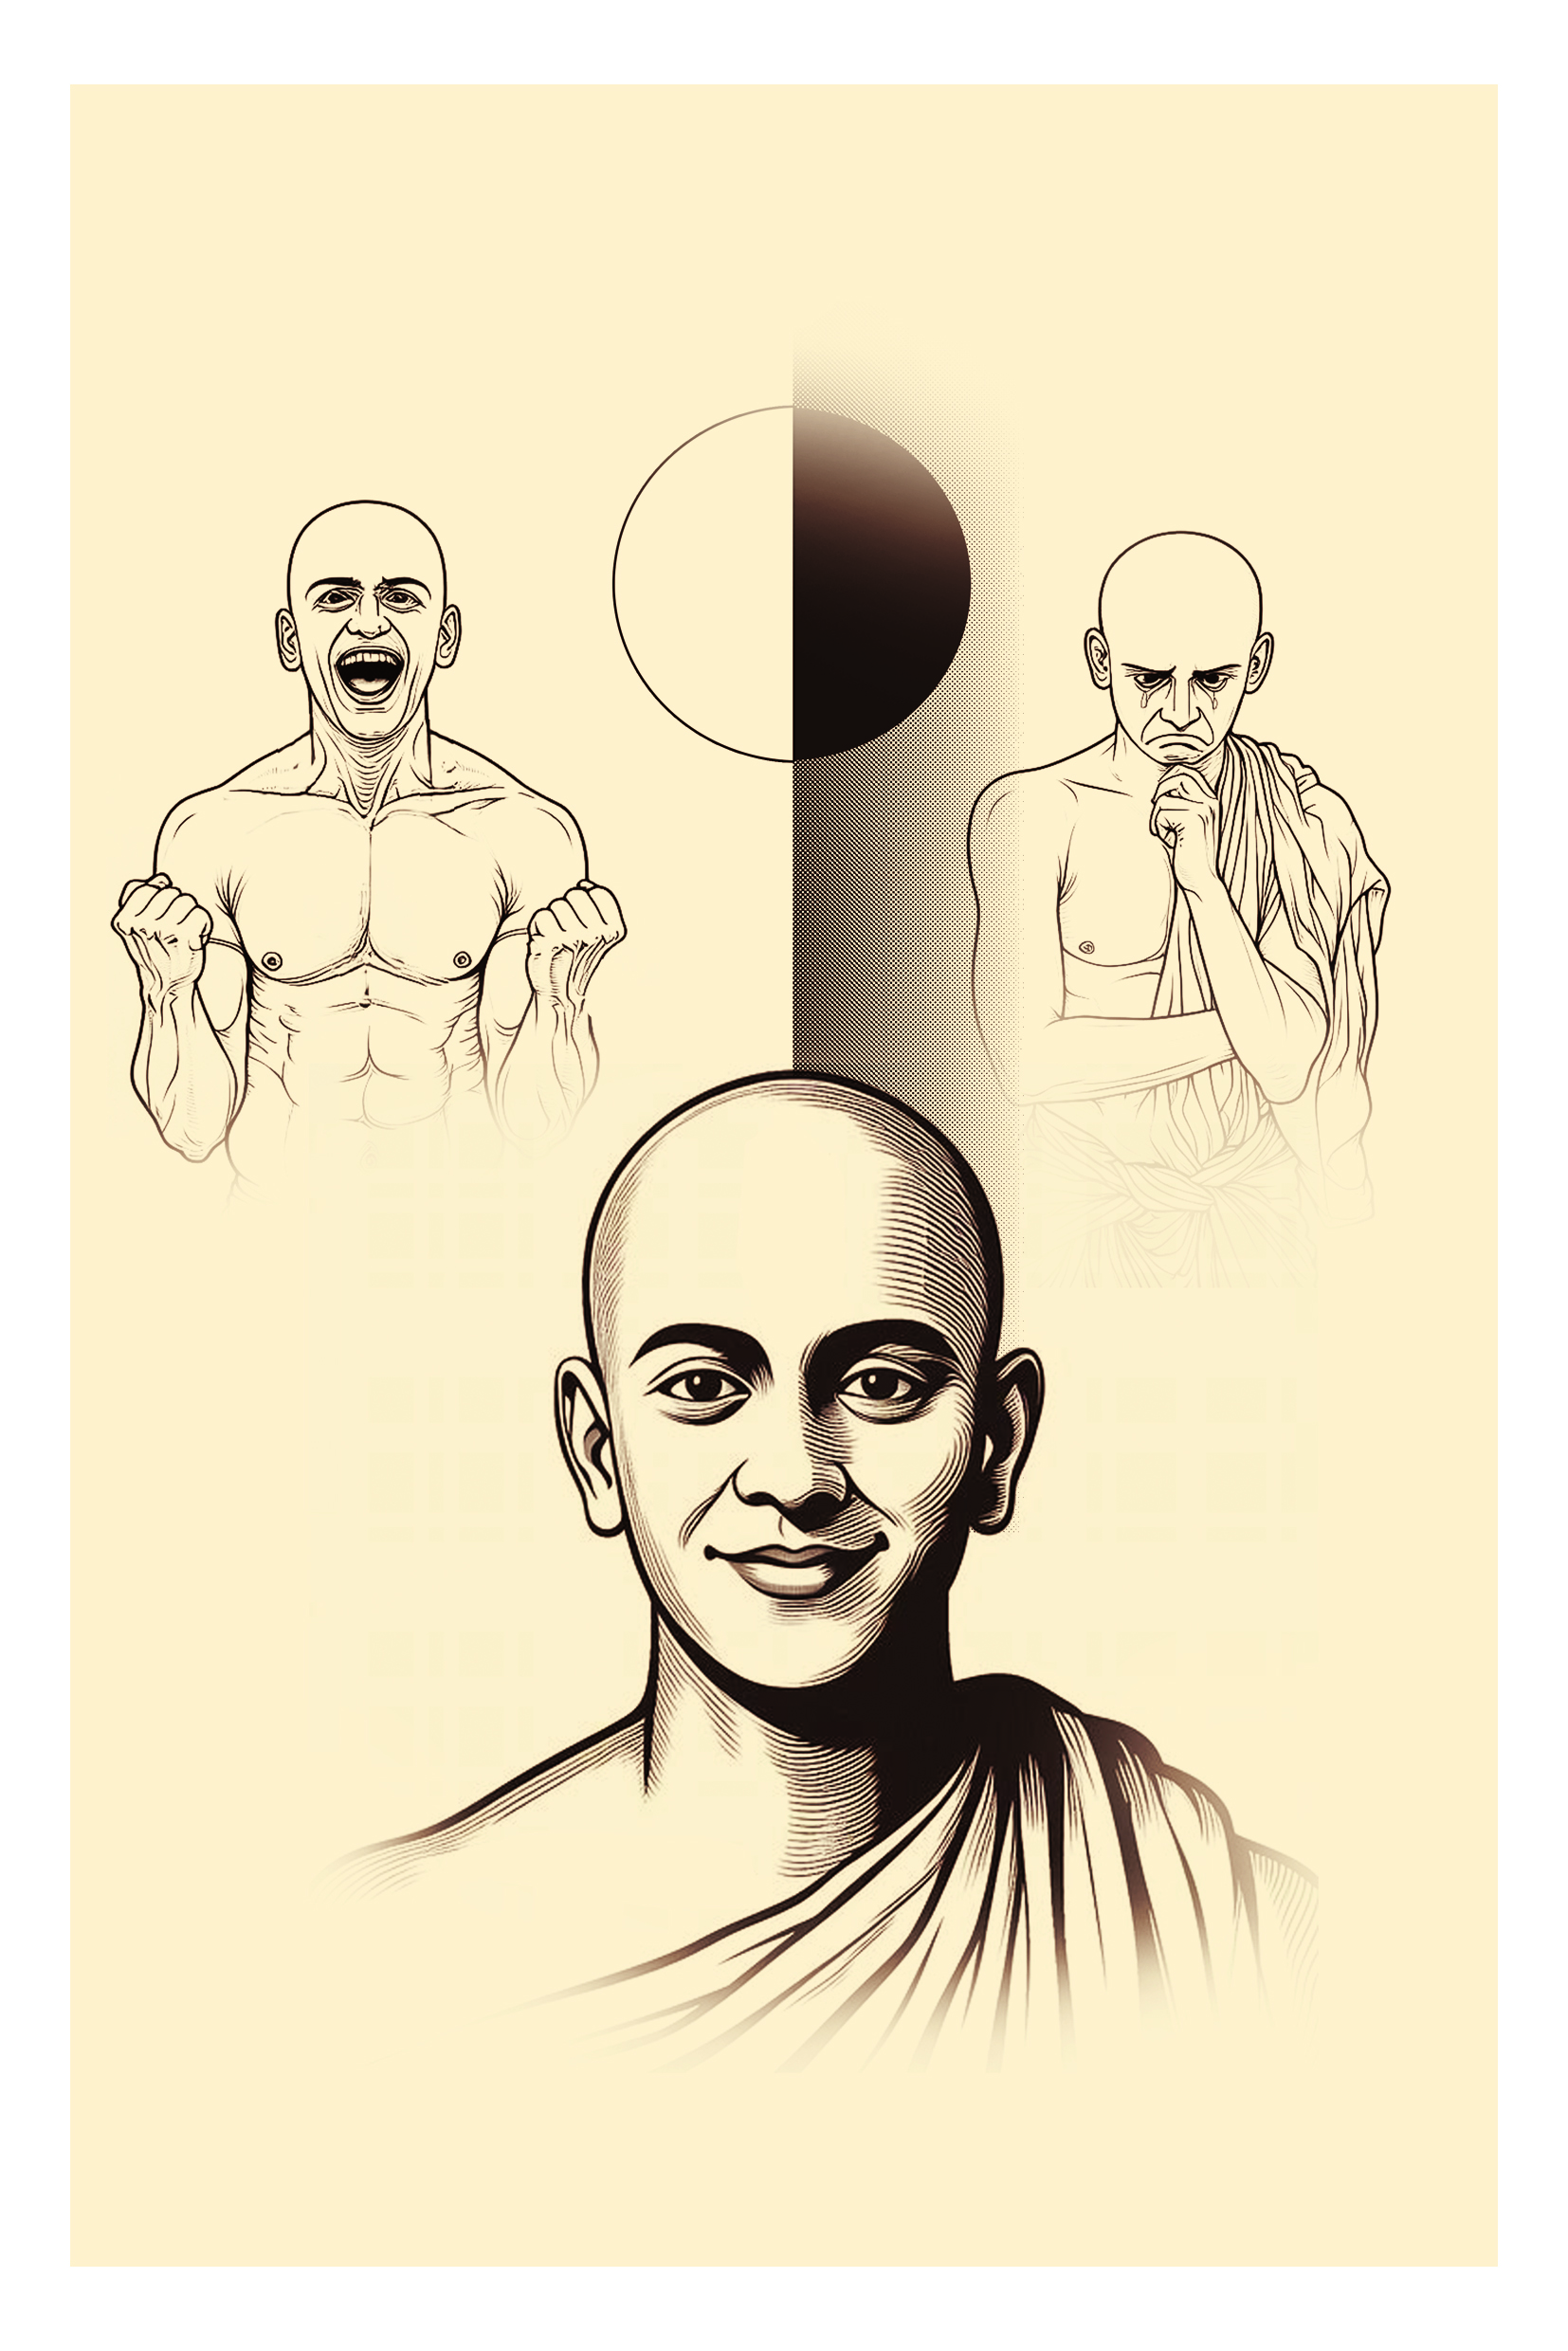
\includegraphics[width=\paperwidth, height=\paperheight, keepaspectratio]{./images/003.jpg}
\end{figure}
\restoregeometry % Restore original geometry settings
\newpage

\begin{mananam}{\mananamfont ಮನನ ಶ್ಲೋಕ - ೪೪}
\small \mananatext ಒಳ್ಳೆಯದು,ಕೆಟ್ಟದ್ದು, ಸುಂದರ, ಕೊಳಕು, ಬಿಳಿ ಮತ್ತು ಕಪ್ಪು ಈ ಮುಂತಾದ ವಿರುದ್ಧ ಜೋಡಿ ಪದಗಳ ಭಾವದಿಂದ ನನ್ನ ಜೀವನದ ದೃಷ್ಟಿಕೋನವು ಕಳಂಕಿತವಾಗಿದೆಯೇ? ನಾನು, ಸದಾ ಇತರರ ಬಗ್ಗೆ ಮತ್ತು ನನ್ನ ಬಗ್ಗೆ ವಿಮರ್ಶಾತ್ಮಕವಾಗಿದ್ದೇನೆಯೇ? ನನ್ನೊಳಗಿನ ಮತ್ತು ಇತರರೊಂದಿಗಿನ  ಸಂಘರ್ಷಕ್ಕೆ ಮೂಲಕಾರಣವಾಗಿರುವ, ವಿಪರೀತ ದೃಷ್ಟಿಕೋನಗಳಿಗೆ ನಾನು ಅಂಟಿಕೊಂಡಿದ್ದೇನೆಯೇ? ತಟಸ್ಥತೆಯ ನಿಲುವನ್ನೂ ತಳೆಯದೇ, ಈ ಎಲ್ಲಾ ಅನಿಸಿಕೆಗಳೂ ಮತ್ತು ವಿಮರ್ಶೆಗಳನ್ನೂ ಮೀರಿ ನಿಲ್ಲುವ ಧೈರ್ಯವಿದೆಯೇ? ಹೀಗಿದ್ದರೂ ಕೂಡ,  ತೆರೆದ ಮನಸ್ಸು ಮತ್ತು ಸ್ವೀಕಾರ ಮನೋಭಾವದಿಂದ ಒಂದು ಉನ್ನತ ಆಯಾಮಕ್ಕೆ ತೆರೆದುಕೊಳ್ಳಬಲ್ಲೆನೇ?
\end{mananam}
\WritingHand\enspace\textbf{ಆತ್ಮ ವಿಮರ್ಶೆ}
\begin{inspiration}{\mananamfont ಸ್ಪೂರ್ತಿ}
\small \mananatext ಎಲ್ಲಾ ಒತ್ತಡದ ಮತ್ತು ಆತಂಕಗಳಿಂದ ನಿಮ್ಮನ್ನು ನೀವು ಮುಕ್ತಗೊಳಿಸಲು ತಕ್ಷಣದ ಮಾರ್ಗವೆಂದರೆ, ನಿಮ್ಮ ದಿನಚರಿಯಲ್ಲಿ ಕೆಲವು ನಿಮಿಷಗಳ ಕಾಲ ದೇಹಕ್ಕೆ ಮತ್ತು ಮನಸ್ಸಿಗೆ, ಅವುಗಳ ನೈಸರ್ಗಿಕ ಸ್ಥಿತಿಯಲ್ಲಿ ವಿಶ್ರಾಂತಿ ಕೊಡಬೇಕು,  ಅಂದರೆ,  ಏನನ್ನೂ ಮಾಡಲು ಬಯಸದೇ ಇರುವುದು ಮತ್ತು ಏನನ್ನೂ ಮಾಡದೇ ಇರುವುದು. ಈ ಸ್ಥಿತಿಯು ಧ್ಯಾನವೂ ಅಲ್ಲ ಅಥವಾ ನಿದ್ರಿಸುವುದೂ ಅಲ್ಲ.ಇದು, ನಿಮ್ಮ ಆತ್ಮದೊಂದಿಗೆ ನೀವು ಇರುವ ಅತೀ ಸಹಜ ಸ್ಥಿತಿ;   ಅಲ್ಲದೇ ಇದು, ಆಳವಾಗಿ ತೃಪ್ತಿ ದಾಯಕವಾದ ಸ್ಥಿತಿಯೂ ಆಗಿದೆ. ಸದಾ ನಮ್ಮನ್ನು ಬಾಹ್ಯ ಪ್ರಪಂಚದಲ್ಲಿಯೇ ತೊಡಗಿಸುವ, ತ್ರಿಗುಣಗಳಾದ ಸತ್ವ, ರಜಸ್, ತಮಸ್ ಗಳಿಂದ ಈ ಸ್ಥಿತಿಯು ( ಆತ್ಮದ ಸಹಜ ಸ್ಥಿತಿ ) ಮುಕ್ತವಾಗಿದೆ. 
\end{inspiration}
\newpage

\newpage
\begin{mananam}{\mananamfont{ಮನನ ಶ್ಲೋಕ - ೪೭,೪೮}}
\small \mananatext ಯಾವುದೇ ಒಂದು ಕಾರ್ಯವನ್ನು, ಪ್ರತಿಫಲಾಪೇಕ್ಷೆ ಇಲ್ಲದೆಯೇ, ಸಮಚಿತ್ತತಾ ಭಾವನೆಯಿಂದ  ಮಾಡಬಲ್ಲೆನೇ? ವಿಶೇಷವಾಗಿ,  ಅಹಿತಕರ ಫಲ ದೊರೆತಾಗಲೂ ಸಹ ಸಮಚಿತ್ತತೆ ಕಾಪಾಡಿಕೊಳ್ಳಬಲ್ಲೆನೇ; ಅಂಥಹ ಭಾವನೆಯ ಆಳವನ್ನಾದರೂ ತಿಳಿಯುವ ಕ್ಷಮತೆ ನನ್ನಲ್ಲಿದೆಯೇ? ಹೆಚ್ಚಿನವರಂತೆ,ಈ ಸಮಾಜದಲ್ಲಿ ನಾನೂ ಕೂಡ, ಎಲ್ಲಾ ಸಂಬಂಧಗಳನ್ನೂ ವ್ಯಾವಹಾರಿಕ ದೃಷ್ಟಿಕೋನದಿಂದ ನೋಡುತ್ತೇನೆಯೇ? ಯಾರಿಂದಲೂ ಏನನ್ನೂ ತೆಗೆದುಕೊಳ್ಳಲು ಬಯಸದೇ, ಏನನ್ನೂ ನಿರೀಕ್ಷಿಸದೇ ನಾನು,  ಕೊಡುವುದನ್ನು ಮಾತ್ರ ಅಭ್ಯಾಸಮಾಡಬಲ್ಲೆನೇ? ‘ಏನನ್ನೂ ತೆಗೆದುಕೊಳ್ಳದೆಲೇ, ಮಾತ್ರ ಕೊಡುವ’, ಈ ತತ್ವವನ್ನು, ನನ್ನ ಜೀವನದಲ್ಲಿ ದೊಡ್ಡ ದೊಡ್ಡ ವಿಷಯಗಳಿಗೆ, ಹಿತಕರವಾಗಿ ಅಳವಡಿಸಿಕೊಳ್ಳುವ  ಮೊದಲು, ನನ್ನ ದಿನನಿತ್ಯ ಜೀವನದಲ್ಲಿ, ಯಾವ, ಯಾವ ಸಣ್ಣ ಪುಟ್ಟ ವಿಷಯಗಳಲ್ಲಿ, ಈ ತತ್ವವನ್ನು ಅಳವಡಿಸಿ ಅಭ್ಯಾಸ ಮಾಡಬಹುದು? 
\end{mananam}
\WritingHand\enspace\textbf{ಆತ್ಮ ವಿಮರ್ಶೆ}
\begin{inspiration}{\mananamfont ಸ್ಪೂರ್ತಿ}
\small \mananatext ಮನಸ್ಸಿನ ಸಮತ್ವವನ್ನು ಸಾಧಿಸಲು ಎಲ್ಲಾ ನಿರೀಕ್ಷೆಗಳಿಂದ ಮನಸ್ಸನ್ನು ಶುದ್ಧೀಕರಿಸುವುದು ಅತ್ಯಗತ್ಯ. ದಿನನಿತ್ಯದ ಜೀವನದಲ್ಲಿ ಮನಸ್ಸಿನ ಈ ಸಮತ್ವವನ್ನು ಕಾಪಾಡಿಕೊಳ್ಳುವುದೇ 'ಯೋಗ' ಮತ್ತು ಈ ಸ್ಥಿತಿಯನ್ನು ಯಾರು ಸಾಧಿಸುತ್ತಾರೋ ಅವನೇ 'ಯೋಗಿ'.
\end{inspiration}
\newpage

\slcol{\Index{ದೂರೇಣ ಹ್ಯವರಂ ಕರ್ಮ} ಬುದ್ಧಿಯೋಗಾದ್ಧನಂಜಯ ।\\
ಬುದ್ಧೌ ಶರಣಮನ್ವಿಚ್ಛ ಕೃಪಣಾಃ ಫಲಹೇತವಃ ॥ ೪೯ ॥}
\cquote{ಅರ್ಜುನ, ಇಂತಹ ಜ್ಞಾನಮಾರ್ಗಕ್ಕಿಂತ ಫಲವನ್ನು ಬಯಸಿ ಮಾಡುವ ಕರ್ಮವು ಬಹು ಕೀಳು. ಅದ್ದರಿಂದ ಜ್ಞಾನ ಯೋಗವನ್ನು ಆಶ್ರಯಿಸು, ಫಲಕ್ಕಾಗಿ ಕರ್ಮ ಮಾಡುವವರು ಶೋಚನೀಯರು.\\}
\slcol{\Index{ಬುದ್ಧಿಯುಕ್ತೋ ಜಹಾತೀಹ} ಉಭೇ ಸುಕೃತದುಷ್ಕೃತೇ ।\\
ತಸ್ಮಾದ್ಯೋಗಾಯ ಯುಜ್ಯಸ್ವ ಯೋಗಃ ಕರ್ಮಸು ಕೌಶಲಮ್ ॥ ೫೦ ॥}
\cquote{ಸಮತ್ವ ಬುದ್ಧಿಯುಕ್ತನು ಬದುಕಿರುವಾಗಲೇ ಪುಣ್ಯ, ಪಾಪ ಎರಡಕ್ಕೂ ಅತೀತನಾಗಬಲ್ಲನು. ಆದ್ದರಿಂದ ಆ ಯೋಗವನ್ನು ಆಶ್ರಯಿಸುವುದಕ್ಕೆ ಯತ್ನ 
ಮಾಡು.\\}
\slcol{\Index{ಕರ್ಮಜಂ ಬುದ್ಧಿಯುಕ್ತಾ} ಹಿ ಫಲಂ ತ್ಯಕ್ತ್ವಾ ಮನೀಷಿಣಃ ।\\
ಜನ್ಮಬಂಧವಿನಿರ್ಮುಕ್ತಾಃ ಪದಂ ಗಚ್ಛಂತ್ಯನಾಮಯಮ್ ॥ ೫೧ ॥}
\cquote{ಜ್ಞಾನಿಗಳು ಕರ್ಮದ ಫಲವನ್ನು ಬಯಸದೆ ಜ್ಞಾನಮಾರ್ಗದಲ್ಲಿ ನಿರತರಾಗಿ ಬಾಳಬಂಧನವನ್ನು ಕಳಚಿಕೊಂಡು ದೋಷದೂರವಾದ ಪರಮ ಪದವಿಯನ್ನು ಪಡೆಯುತ್ತಾರೆ.\\}
\slcol{\Index{ಯದಾ ತೇ ಮೋಹಕಲಿಲಂ} ಬುದ್ಧಿರ್ವ್ಯತಿತರಿಷ್ಯತಿ ।\\
ತದಾ ಗಂತಾಸಿ ನಿರ್ವೇದಂ ಶ್ರೋತವ್ಯಸ್ಯ ಶ್ರುತಸ್ಯ ಚ ॥ ೫೨ ॥}
\cquote{ನಿನ್ನ ಮನಸ್ಸು ತಪ್ಪು ತಿಳಿವೆಂಬ ಹೊಲಸನ್ನು ಕಳೆದುಕೊಂಡಾಗ ನೀನು ಕೇಳಿದ, ಕೇಳಲಿರುವ ಎಲ್ಲ ಉಪದೇಶ ಸಾರ್ಥಕವಾಗುತ್ತದೆ.\\}
\slcol{\Index{ಶ್ರುತಿವಿಪ್ರತಿಪನ್ನಾ ತೇ} ಯದಾ ಸ್ಥಾಸ್ಯತಿ ನಿಶ್ಚಲಾ ।\\
ಸಮಾಧಾವಚಲಾ ಬುದ್ಧಿಸ್ತದಾ ಯೋಗಮವಾಪ್ಸ್ಯಸಿ ॥ ೫೩ ॥}
\cquote{ವೇದವಾದಗಳಿಂದ ಚಂಚಲವಾಗಿರುವ ನಿನ್ನ ಬುದ್ಧಿಯು ವಿಷಯಗಳಿಗೆರಗದೆ,ಅಲುಗಾಡದೆ ಆತ್ಮನಲ್ಲಿ ನೆಲೆಯಾಗಿ ನಿಂತಾಗ ಆತ್ಮದೊಡನೆ ಕೂಡಿದವನಾಗಿರುವೆ.\\}
\slcol{ಅರ್ಜುನ ಉವಾಚ ।\\
\Index{ಸ್ಥಿತಪ್ರಙ್ಞಸ್ಯ ಕಾ ಭಾಷಾ} ಸಮಾಧಿಸ್ಥಸ್ಯ ಕೇಶವ ।\\
ಸ್ಥಿತಧೀಃ ಕಿಂ ಪ್ರಭಾಷೇತ ಕಿಮಾಸೀತ ವ್ರಜೇತ ಕಿಮ್ ॥ ೫೪ ॥}
\cquote{ಅರ್ಜುನನು ಹೇಳಿದನು, ಕೇಶವ ಸಮಾಧಿನಿಷ್ಠನಾದ ಸ್ಥಿತಪ್ರಜ್ಞನ ಲಕ್ಷಣವೇನು? ಅವನು ಹೇಗೆ ಮಾತನಾಡುತ್ತಾನೆ? ಹೇಗೆ ಇರುತ್ತಾನೆ? ಹೇಗೆ 
ವ್ಯವಹರಿಸುತ್ತಾನೆ?\\}
\slcol{ಶ್ರಿ\!\char"0CD5ಭಗವಾನುವಾಚ।\\
\Index{ಪ್ರಜಹಾತಿ ಯದಾ ಕಾಮಾನ್ಸ}ರ್ವಾನ್ಪಾರ್ಥ ಮನೋಗತಾನ್ ।\\
ಆತ್ಮನ್ಯೇವಾತ್ಮನಾ ತುಷ್ಟಃ ಸ್ಥಿತಪ್ರಙ್ಞಸ್ತದೋಚ್ಯತೇ ॥ ೫೫ ॥}
\cquote{ಅರ್ಜುನಾ, ಮನಸ್ಸಿನಲ್ಲಿರುವ ಬಯಕೆಗಳನ್ನೆಲ್ಲ ಬಿಟ್ಟಾಗ ಅವನು ತನ್ನಿಂದಲೇ ತನ್ನಲ್ಲಿ ತೃಪ್ತನಾಗಿ ಆತ್ಮದಲ್ಲಿ ಸ್ಥಿರವಾದ ಬುದ್ಧಿಯುಳ್ಳವನಾಗುತ್ತಾನೆ.}

\newpage
\begin{mananam}{\mananamfont ಮನನ ಶ್ಲೋಕ - ೫೦}
\small \mananatext ನನ್ನ ಬಾಹ್ಯಜೀವನದಲ್ಲಿ ಮಾತ್ರವಲ್ಲ ನನ್ನ ಆಂತರಿಕ ಜೀವನದಲ್ಲಿಯೂ ಯಶಸ್ವಿಯಾಗಲು ಅಗತ್ಯವಾದ ಕೌಶಲ್ಯಗಳನ್ನು ಹೊಂದಿದ್ದೇನೆಯೇ? ವಿಶೇಷವಾಗಿ ಕೆಲಸದ ಒತ್ತಡ ಇರುವಾಗ ನನ್ನ ಭಾವನೆಗಳನ್ನು ನಿಭಾಯಿಸುವ ಸಾಮರ್ಥ್ಯವಿದೆಯೇ? ನನ್ನ ಎಲ್ಲಾ ಸಂಬಂಧಗಳಲ್ಲಿ ನಾನು  ಸಾಮರಸ್ಯದಿಂದ ಇರಲು ಸಾಧ್ಯವೇ? ನನ್ನ ಸಮತೋಮುಖ ಯೋಗಕ್ಷೇಮಕ್ಕಾಗಿ ಮಾಡುವ ಪ್ರಯತ್ನಗಳಲ್ಲಿ ತಾಳ್ಮೆ ಮತ್ತು ನಿರಂತರತೆಯನ್ನು ಹೊಂದಿರಲು ಸಾಧ್ಯವೇ? ಗೀತೆಯ ದೃಷ್ಟಿ ಕೋನದಂತೆ ಈ ಲೌಕಿಕ ಲಾಭ ನಷ್ಟವನ್ನು ಮೀರಿ, ಮಾನಸಿಕ ಸಮತ್ವದ ಸ್ಥಿತಿ ಪಡೆಯಲು ಬೇಕಾದ ಗೀತೆಯ ದೃಷ್ಟಿಕೋನ ನನಗಿದೆಯೇ?
\end{mananam}
\WritingHand\enspace\textbf{ಆತ್ಮ ವಿಮರ್ಶೆ}
\begin{inspiration}{\mananamfont ಸ್ಪೂರ್ತಿ}
\small \mananatext ಯೋಗಭ್ಯಾಸದ ಉದ್ದೇಶವು, ಜೀವನಕ್ಕೆ ಅಗತ್ಯವಾದ ಕೌಶಲ್ಯಗಳೊಂದಿಗೆ ನಮ್ಮನ್ನು ಸಜ್ಜುಗೊಳಿಸುವುದು. ಒಂದು ವಾಹನವನ್ನು ಓಡಿಸಲು ಕೌಶಲ್ಯಗಳು ಹೇಗೆ ಬೇಕೋ ಹಾಗೆಯೇ, ಜೀವನ ನಿರ್ವಹಿಸಲು ನಮಗೆ ಜೀವನ ಕೌಶಲ್ಯಗಳು ಬೇಕಾಗುತ್ತವೆ.ಕೌಶಲ್ಯದಿಂದ, ಅರ್ಪಣಾ ಮನೋಭಾವದಿಂದ, ಪ್ರತಿಫಲಾಪೇಕ್ಷೆ ಇಲ್ಲದೆಯೇ ಕೆಲಸ ಮಾಡುವುದರಿಂದ, ಒಬ್ಬ ಕರ್ಮಯೋಗಿಯು, ಕ್ರಿಯೆಗಳಿಂದ ಪ್ರೇರಿತವಾದ ಬಂಧನದಿಂದ ಮುಕ್ತನಾಗುತ್ತಾನೆ.
\end{inspiration}
\newpage



\newpage
\begin{mananam}{\mananamfont{ಮನನ ಶ್ಲೋಕ - ೫೨, ೫೩}}
\small \mananatext ನನ್ನ ಮನಸ್ಸು ಯೋಗ ಮಾರ್ಗದಲ್ಲಿ ಸಲ್ಪ ಮಟ್ಟಿಗಿನ ಸ್ಥಿರತೆ ಸಾಧಿಸಿದೆಯೇ? ಈ ಮಾರ್ಗದಲ್ಲಿ ಇನ್ನೂ ನಾನು, ಅಸ್ಪಷ್ಟ  ಮತ್ತು ಗೊಂದಲದಲ್ಲಿದ್ದೇನೆಯೇ? ಅನುಮಾನಗಳನ್ನು ಪರಿಹರಿಸಿಕೊಳ್ಳಲು ನನ್ನ ಬಳಿ ಯಾವುದಾದರೂ ಮಾರ್ಗವಿದೆಯೇ? ಇದಕ್ಕೆ ಆಧಾರ ಯಾವುದು? ಬೋಧನೆಯೇ ಅಥವಾ ಶಿಕ್ಷಕನೇ? ಯಾವುದನ್ನು ಆಶ್ರಯಿಸುತ್ತೇನೆ? ಈ ಬಾಹ್ಯ ಆಶ್ರಯಗಳ ಮೂಲಕ, ನನ್ನ ಒಳಗಿರುವ ಗುರುತತ್ವದೊಂದಿಗೆ ಹೆಚ್ಚಿನ ತಲ್ಲೀನತೆ ಹೊಂದುತ್ತಿರುವ ಭಾವನೆ ಇದೆಯೇ?
\end{mananam}
\WritingHand\enspace\textbf{ಆತ್ಮ ವಿಮರ್ಶೆ}
\begin{inspiration}{\mananamfont ಸ್ಪೂರ್ತಿ}
\small \mananatext ಭ್ರಮೆಯಿಂದ ನಮ್ಮನ್ನು ಕದಲಿಸಿ ಹೊರ ತರುವುದೇ ಗುರುಗಳ ಮತ್ತು ಪುರಾಣ ಗ್ರಂಥಗಳ ಉದ್ದೇಶ. ಗೊಂದಲಗಳು ಮತ್ತು ಸವಾಲುಗಳು ಅಧ್ಯಾತ್ಮ ಪ್ರಯಾಣದ ಒಂದು ಭಾಗವಾಗಿದೆ. ಲೌಕಿಕ ಚಿಂತನೆಗಳನ್ನು ದೂರಸರಿಸಿದರೆ ಉನ್ನತ ವಾಸ್ತವದಲ್ಲಿ ಆಶ್ರಯ ಪಡೆಯಬಹುದು. ಹೀಗೆ ನಾವು ಪ್ರಗತಿ ಹೊಂದಿದಾಗ ಈ ಮಾರ್ಗದಲ್ಲಿ ಸ್ಪಷ್ಟತೆಯನ್ನು ಪಡೆಯುತ್ತೇವೆ.
\end{inspiration}
\newpage


\newpage
\begin{mananam}{\mananamfont ಮನನ ಶ್ಲೋಕ - ೫೪}
\small \mananatext ಸಾಕ್ಷಾತ್ಕಾರದ ಸ್ಥಿತಿ ಯಾವುದು ಎಂದು ನಾನು ಅರ್ಥ ಮಾಡಿಕೊಂಡಿದ್ದೇನೆಯೇ? ಸಂತರ,  ಸಾಕ್ಷಾತ್ಕಾರದ  ವಿವಿಧ ಹಂತಗಳ ಬಗ್ಗೆ ನನಗೆ ತಿಳಿದಿದೆಯೇ? ನನ್ನ ಸ್ವಂತ ಅಧ್ಯಾತ್ಮಿಕ ವಿಕಾಸದ ಮುಂದಿನ ಹಂತ ಯಾವುದು? ನಾನು ಯಾವ ಹಂತವನ್ನು ಪ್ರಾಮಾಣಿಕವಾಗಿ ಬಯಸಬಹುದು? ಅಂತಿಮ ವಿಮೋಚನೆ ಮತ್ತು ಸ್ವಾತಂತ್ರ್ಯದ ಬಗೆಗಿನ ನನ್ನ ತಿಳುವಳಿಕೆಯು,  ನನ್ನ ಜೀವನದಲ್ಲಿ ಮಾನಸಿಕ ಮತ್ತು ಅಧ್ಯಾತ್ಮಿಕ ಪ್ರಗತಿಯನ್ನು ಮಾಡಲು  ನನ್ನನ್ನು ಪ್ರೇರೇಪಿಸುತ್ತದೆಯೇ?
\end{mananam}
\WritingHand\enspace\textbf{ಆತ್ಮ ವಿಮರ್ಶೆ}
\begin{inspiration}{\mananamfont ಸ್ಪೂರ್ತಿ}
\small \mananatext ಜೀವನದ ಪ್ರತಿಯೊಂದು ಕ್ಷೇತ್ರದಲ್ಲೂ,  ಯಶಸ್ವಿಯಾದ ಜನರಿಂದ ನಾವು ಪ್ರೇರಿತರಾಗಿದ್ದೇವೆ. ಹಾಗೆಯೇ, ಸಾಧು, ಸಂತರು ಸಾಧಿಸಿದ ಭಾಹ್ಯಸ್ಥಿತಿ ಮಾತ್ರವಲ್ಲ, ಆಂತರಿಕ ಸ್ಥಿತಿಯ ಬಗ್ಗೆಯೂ ಬಹಳಷ್ಟು ಜನರಿಗೆ ಅರ್ಥೈಸಿಕೊಳ್ಳಲು ಕಷ್ಟವಾಗುತ್ತದೆ. ಅವರ ಈ ಆಂತರಿಕ ಸ್ಥಿತಿಯನ್ನು ಚೆನ್ನಾಗಿ ಅರ್ಥೈಸಿಕೊಳ್ಳುವುದರಿಂದ, ತಪ್ಪು ತಿಳುವಳಿಕೆ ಮತ್ತು ತಪ್ಪು ನಿರ್ಧಾರಗಳಿಂದ ದೂರವಿರಲು ಸಹಾಯವಾಗುತ್ತದೆ.
\end{inspiration}
\newpage



\newpage
\begin{mananam}{\mananamfont ಮನನ ಶ್ಲೋಕ - ೫೫}
\small \mananatext ಅಧ್ಯಾತ್ಮಿಕ ಪ್ರಗತಿಯಾಗದಂತೆ ನನ್ನನ್ನು ತಡೆಯುತ್ತಿರುವ ಕೆಳಮಟ್ಟದ ಆಸೆಗಳು ಯಾವುವು? ನನ್ನನ್ನು ಕೆಳಮಟ್ಟಕ್ಕೆ ಎಳೆಯುತ್ತಿರುವ ಮಾನಸಿಕ ಅಭ್ಯಾಸಗಳು ಮತ್ತು ಭಾವೋದ್ರೇಕಗಳನ್ನು   ನಾನು ಹೇಗೆ ತ್ಯಜಿಸಬಹುದು? ಆನಂದ ಮತ್ತು ತೃಪ್ತಿಯನ್ನು ಒಬ್ಬನ ಸ್ವಂತ ಆತ್ಮದಲ್ಲಿಯೇ ಕಂಡುಕೊಳ್ಳುವುದು ಎಂಬುದರ ಅರ್ಥವೇನು?
\end{mananam}
\WritingHand\enspace\textbf{ಆತ್ಮ ವಿಮರ್ಶೆ}
\begin{inspiration}{\mananamfont ಸ್ಪೂರ್ತಿ}
\small \mananatext  ಒಬ್ಬ ನಿಜವಾದ ಯೋಗಿ ಅಥವಾ ಸoನ್ಯಾಸಿಯು ಯಾರೆಂದರೆ, ತನ್ನ ಸಂತೋಷಕ್ಕಾಗಿ, ಯಾವುದರ ಮೇಲೆಯೂ ಅಥವಾ ಯಾರ ಮೇಲೆಯೂ ಅವಲಂಬಿತನಾಗದಿದ್ದವನು. ತನ್ನ ಸ್ವಂತ ಆತ್ಮದಲ್ಲಿಯೇ ಸುಖ ಮತ್ತು ಸಂತೋಷ ಕಂಡುಕೊಂಡಿರುವ ಇವನು, ಯಾವುದೇ ಲೌಕಿಕ ಆಸೆಗಳಿಗೂ ಹಾತೊರೆಯುವುದಿಲ್ಲ.
\end{inspiration}
\newpage

\slcol{\Index{ದುಃಖೇಷ್ವನುದ್ವಿಗ್ನಮನಾಃ} ಸುಖೇಷು ವಿಗತಸ್ಪ\,\char"0CC3ಹಃ ।\\
ವೀತರಾಗಭಯಕ್ರೋಧಃ ಸ್ಥಿತಧೀರ್ಮುನಿರುಚ್ಯತೇ ॥ ೫೬ ॥}
\cquote{ದುಃಖಗಳು ಬಂದಾಗ ತಳವಳಗೊಳ್ಳದೆ, ಸುಖಗಳ ಬಗೆಗೆ ಇಚ್ಛೆ ಇಲ್ಲದೆ, ಒಲವು, ಹೆದರಿಕೆ, ಸಿಟ್ಟು ಇಂಥ ಭಾವಗಳಿಗೆ ಬಲಿಯಾಗದೆ ಆತ್ಮವಿಚಾರವನ್ನೇ ಹಚ್ಚಿಕೊಂಡಿರುವವನು ಸ್ಥಿತಪ್ರಜ್ಞ ಎನಿಸಿಕೊಳ್ಳುತ್ತಾನೆ.\\}
\slcol{\Index{ಯಃ ಸರ್ವತ್ರಾನಭಿಸ್ನೇಹ}ಸ್ತತ್ತತ್ಪ್ರಾಪ್ಯ ಶುಭಾಶುಭಮ್ ।\\
ನಾಭಿನಂದತಿ ನ ದ್ವೇಷ್ಟಿ ತಸ್ಯ ಪ್ರಙ್ಞಾ ಪ್ರತಿಷ್ಠಿತಾ ॥ ೫೭ ॥}
\cquote{ಯಾವುದನ್ನೂ ಅತಿಯಾಗಿ ಹಚ್ಚಿಕೊಳ್ಳದೆ, ಒಳ್ಳೆಯದೂ, ಕೆಟ್ಟದ್ದೂ ಒದಗಿ ಬಂದಾಗ ಹಿಗ್ಗದೇ, ಕುಗ್ಗದೇ ಸಮವಾಗಿ ಕಾಣಬಲ್ಲವನ ಪ್ರಜ್ಞೆ ಸ್ಥಿರವಾಗಿರುತ್ತದೆ.\\}
\slcol{\Index{ಯದಾ ಸಂಹರತೇ ಚಾಯಂ} ಕೂರ್ಮೋऽಂಗಾನೀವ ಸರ್ವಶಃ ।\\
ಇಂದ್ರಿಯಾಣೀಂದ್ರಿಯಾರ್ಥೇಭ್ಯಸ್ತಸ್ಯ ಪ್ರಙ್ಞಾ ಪ್ರತಿಷ್ಠಿತಾ ॥ ೫೮ ॥}
\cquote{ಆಮೆಯು ತನ್ನ ಅವಯವಗಳನ್ನು ಎಲ್ಲ ಕಡೆಯಿಂದಲೂ ಒಳ ಸೆಳೆದುಕೊಳ್ಳುವಂತೆ ಹೊರಗಣ ವಿಷಯಗಳಿಂದ ಇಂದ್ರಿಯಗಳನ್ನು ಅಂತರ್ಮುಖಗೊಳಿಸಬಲ್ಲವನ ಪ್ರಜ್ಞೆ ಸ್ಥಿರವಾಗಿರುತ್ತದೆ.\\}
\slcol{\Index{ವಿಷಯಾ ವಿನಿವರ್ತಂತೇ} ನಿರಾಹಾರಸ್ಯ ದೇಹಿನಃ ।\\
ರಸವರ್ಜಂ ರಸೋऽಪ್ಯಸ್ಯ ಪರಂ ದೃ\char"0CB7\char"0CCD\char"0C9F\char"0CBE\;\char"0CCD\char"0CB5\enspace ನಿವರ್ತತೇ ॥ ೫೯ ॥}
\cquote{ಆಹಾರ ನಿಗ್ರಹದಿಂದ ಜೀವನಿಗೆ ವಿಷಯ ಭೋಗದ ಶಕ್ತಿ ಕುಂದುವುದೇ ಹೊರತು ಭೋಗದ ಬಯಕೆ ಕುಂದುವುದಿಲ್ಲ. ಭಗವಂತನ ದರ್ಶನವಾದಾಗಲೇ ಈ ಬಯಕೆಯನ್ನೂ ನಿಗ್ರಹಿಸುವುದು ಸಾಧ್ಯ.\\}
\slcol{\Index{ಯತತೋ ಹ್ಯಪಿ ಕೌಂತೇಯ} ಪುರುಷಸ್ಯ ವಿಪಶ್ಚಿತಃ ।\\
ಇಂದ್ರಿಯಾಣಿ ಪ್ರಮಾಥೀನಿ ಹರಂತಿ ಪ್ರಸಭಂ ಮನಃ ॥ ೬೦ ॥}
\cquote{ಹತ್ತು ಕಡೆಗೂ ಎಳೆಯುವಂತ ಇಂದ್ರಿಯಗಳು ಪ್ರಯತ್ನಿಶೀಲನಾದ ಜ್ಞಾನಿಯ ಮನಸ್ಸನ್ನೂ ಬಲಾತ್ಕಾರವಾಗಿ ಅಪಹರಿಸಿಬಿಡುವವು.\\}
\slcol{\Index{ತಾನಿ ಸರ್ವಾಣಿ ಸಂಯಮ್ಯ} ಯುಕ್ತ ಆಸೀತ ಮತ್ಪರಃ ।\\
ವಶೇ ಹಿ ಯಸ್ಯೇಂದ್ರಿಯಾಣಿ ತಸ್ಯ ಪ್ರಙ್ಞಾ ಪ್ರತಿಷ್ಠಿತಾ ॥ ೬೧ ॥}
\cquote{ಅವೆಲ್ಲವನ್ನೂ ಬಿಗಿಹಿಡಿದು ನನ್ನನ್ನೇ ಗತಿಯೆಂದು ನನ್ನಲ್ಲಿಯೇ ಮನಸ್ಸಿಡಬೇಕು. ಯಾರ ಇಂದ್ರಿಯಗಳು ಹಿಡಿತದಲ್ಲಿರುವವೋ ಅವನ ಪ್ರಜ್ಞೆ ಸ್ಥಿರವಾಗಿರುತ್ತದೆ.\\}
\slcol{\Index{ಧ್ಯಾಯತೋ ವಿಷಯಾನ್ಪುಂಸಃ} ಸಂಗಸ್ತೇಷೂಪಜಾಯತೇ ।\\
ಸಂಗಾತ್ಸಂಜಾಯತೇ ಕಾಮಃ ಕಾಮಾತ್ಕ್ರೋಧೋऽಭಿಜಾಯತೇ ॥ ೬೨ ॥}
\cquote{ಸುಖ ಸಾಧನಗಳನ್ನೇ ಹಂಬಲಿಸುತ್ತಿರುವ ಅವನಿಗೆ ಅವುಗಳಲ್ಲಿ ಆಸಕ್ತಿ ಹುಟ್ಟುತ್ತದೆ. ಆಸಕ್ತಿಯಿಂದ ಬಯಕೆ ಹುಟ್ಟುತ್ತದೆ.ಬಯಕೆ ಈಡೇರದಾಗ ಸಿಟ್ಟು ತಲೆ ಹಾಕುತ್ತದೆ.\\}

\newpage
\begin{mananam}{\mananamfont {ಮನನ ಶ್ಲೋಕ - ೫೬, ೫೭}}
\small \mananatext ವೈಫಲ್ಯಗಳು ಮತ್ತು ನಷ್ಟಗಳು ನನ್ನನ್ನು ಮಾನಸಿಕವಾಗಿ  ಕುಗ್ಗಿಸುತ್ತವೆಯೇ? ಅವುಗಳನ್ನು ವೈಯಕ್ತಿಕವಾಗಿ ಪರಿಗಣಿಸುತ್ತೇನೆಯೇ? ಅದು ನನ್ನ ಆತ್ಮವಿಶ್ವಾಸದ ಮೇಲೆ ಪರಿಣಾಮ ಬೀರಲು ನಾನು ಬಿಡುತ್ತೇನೆಯೇ? ಯಶಸ್ಸು ಮತ್ತು ಲಾಭ ಬಂದಾಗ ಹೇಗಿರುತ್ತದೆ? ನಾನು ಅತಿಯಾಗಿ  ಉತ್ಸುಕನಾಗುತ್ತೇನೆಯೇ? ಅದು ನನ್ನನ್ನು ಅಹಂಕಾರಿಯಾಗಿ ಮತ್ತು ಇತರರ ಬಗ್ಗೆ ನಿರಾಕರಣೆ ಭಾವ ಹೊಂದುವಂತೆ ಮಾಡುತ್ತದೆಯೇ? ಜೀವನದ ಸನ್ನಿವೇಶದಲ್ಲಿ, ಇದು ಒಳ್ಳೆಯದು ಅಥವಾ ಕೆಟ್ಟದ್ದು ಎಂದು ನಾನು ನಿರಂತರವಾಗಿ ನಿರ್ಣಯಿಸುತ್ತಾ ಇರುತ್ತೇನೆಯೇ?
\end{mananam}
\WritingHand\enspace\textbf{ಆತ್ಮ ವಿಮರ್ಶೆ}
\begin{inspiration}{\mananamfont ಸ್ಪೂರ್ತಿ}
\small \mananatext ಒಬ್ಬ ಸಾಮಾನ್ಯ ಮನುಷ್ಯನಿಗೆ, ಜೀವನದಲ್ಲಿ ಬರುವ ಸಂದರ್ಭಗಳಿಗೆ ತಕ್ಕಂತೆ ಮಾನಸಿಕ ಸ್ಥಿತಿಯು ಬದಲಾಗುತ್ತಿರುತ್ತದೆ. ಹೀಗಾಗಿ ಜೀವನದಲ್ಲಿ ಧನಾತ್ಮಕ ಫಲಿತಾಂಶಗಳ ಕಡೆಗೆ ಒಲವು ಮತ್ತು ಋಣಾತ್ಮಕ ಫಲಿತಾಂಶಗಳ ಬಗ್ಗೆ ವಿಮುಖತೆಯಾಗುತ್ತದೆ. ಆದರೆ,  ಒಬ್ಬ ಯೋಗಿಗೆ, ತನ್ನ ಎಲ್ಲಾ ಅಧ್ಯಾತ್ಮಿಕ ಅಭ್ಯಾಸದ ಗುರಿ, ಜೀವನದಲ್ಲಿ ಯಾವಾಗಲೂ ಅನುಕೂಲಕರ ಸಂದರ್ಭವನ್ನು ಪಡೆಯುವುದು ಅಲ್ಲ, ಎಂತಹ ಸಂದರ್ಭದಲ್ಲಿಯೂ ಮಾನಸಿಕ ಸ್ಥಿರತೆಯನ್ನು ಪಡೆಯುವುದೇ ಆಗಿದೆ.
\end{inspiration}
\newpage

\begin{mananam}{\mananamfont ಮನನ ಶ್ಲೋಕ - ೫೮}
\small \mananatext ಇಂದ್ರಿಯ ನಿಯಂತ್ರಣಗಳನ್ನು ಎಷ್ಟರ ಮಟ್ಟಿಗೆ ನಾನು ಹೊಂದಿದ್ದೇನೆ? ಇಂದ್ರಿಯ ಸುಖದಲ್ಲಿ ನಾನು ಅತಿಯಾಗಿ ತೊಡಗಿಸಿಕೊಳ್ಳುತ್ತೇನೆಯೇ? ನನ್ನ ಮನಸ್ಸನ್ನು ಇಂದ್ರಿಯಗಳ ಕಡೆಗೆ ಸೆಳೆಯುವ, ಬಾಹ್ಯ ಪ್ರಚೋದನೆಗಳ ಬಗ್ಗೆ ನನಗೆ ಅರಿವಿದೆಯೇ? ಆಕರ್ಷಕ ವಸ್ತುಗಳನ್ನು ಪ್ರಸ್ತುತಪಡಿಸುವ,ನಮ್ಮ ಆಂತರಿಕ ಪ್ರಚೋದನೆಗಳಾದ ಯೋಚನೆಗಳು ಮತ್ತು ನೆನಪುಗಳ ಬಗ್ಗೆ, ನನಗೆ ಅರಿವಿದೆಯೇ? ಇಂದ್ರಿಯಗಳಿಂದ ನನ್ನ ಮನಸ್ಸನ್ನು ಹಿಂತೆಗೆದುಕೊಳ್ಳುವ ಯಾವುದಾದರೂ ವಿಧಾನವನ್ನು ನಾನು ಪ್ರಯತ್ನಿಸಿದ್ದೇನೆಯೇ? ಇಲ್ಲವಾದಲ್ಲಿ, ಅದನ್ನು ಹೇಗೆ ಅಭಿವೃದ್ಧಿಗೊಳಿಸುವುದು?
\end{mananam}
\WritingHand\enspace\textbf{ಆತ್ಮ ವಿಮರ್ಶೆ}
\begin{inspiration}{\mananamfont ಸ್ಪೂರ್ತಿ}
\small \mananatext ಸ್ವಾಭಾವಿಕವಾಗಿ ಹೊರಗೆ ಹೋಗುವ ಇಂದ್ರಿಯಗಳನ್ನು ಒಳಕ್ಕೆ ಹಿಂತೆಗೆದುಕೊಳ್ಳಲು ಪ್ರಜ್ಞಾಪೂರ್ವಕ ತರಬೇತಿಯನ್ನು ಪಡೆಯಬೇಕಾಗುತ್ತದೆ. ವ್ಯಸನಗಳ ಹಾನಿಯ ಬಗ್ಗೆ, ಕೇವಲ ಜ್ಞಾನ ಮತ್ತು ಆಶಯ (ವ್ಯಸನಗಳನ್ನು ಬಿಡಬೇಕೆಂಬ ) ಸಾಕಾಗುವುದಿಲ್ಲ. ಹೊಸತಾಗಿ ಧನಾತ್ಮಕ ಅಭ್ಯಾಸಗಳನ್ನು ಬೆಳೆಸಿಕೊಳ್ಳಲು, ಸತತವಾಗಿ ಆತ್ಮ ಶೋಧನೆಯನ್ನು, ಸ್ವಲ್ಪ ಸ್ವಲ್ಪವಾಗಿ, ಹೆಚ್ಚಳ ಮಾಡುತ್ತಾ ಹೋಗುವ ಕ್ರಮಗಳು ಉತ್ತಮ ವಿಧಾನವಾಗಿರುತ್ತವೆ.
\end{inspiration}
\newpage

\slcol{\Index{ಕ್ರೋಧಾದ್ಭವತಿ ಸಂಮೋಹಃ} ಸಂಮೋಹಾತ್ ಸ್ಮ\,\char"0CC3ತಿವಿಭ್ರಮಃ ।\\
ಸ್ಮ\,\char"0CC3ತಿಭ್ರಂಶಾದ್ಬುದ್ಧಿನಾಶೋ ಬುದ್ಧಿನಾಶಾತ್ಪ್ರಣಶ್ಯತಿ ॥ ೬೩ ॥}
\cquote{ಸಿಟ್ಟಿನ ಮರಿ ಅವಿವೇಕ. ಅವಿವೇಕದಿಂದ ಧರ್ಮ ಅಧರ್ಮಗಳ ಮರೆವು. ಇಂತ ಮರೆವಿನಿಂದ ಬುದ್ಧಿ ಕೆಡುತ್ತದೆ. ಬುದ್ದಿ ಕೆಡುವುದೇ ಎಲ್ಲ ಅನರ್ಥದ ಮೂಲ.\\}
\slcol{\Index{ರಾಗದ್ವೇಷವಿಮುಕ್ತೈಸ್ತು} ವಿಷಯಾನಿಂದ್ರಿಯೈಶ್ಚರನ್ ।\\
ಆತ್ಮವಶ್ಯೈರ್ವಿಧೇಯಾತ್ಮಾ ಪ್ರಸಾದಮಧಿಗಚ್ಛತಿ ॥ ೬೪ ॥}
\cquote{ಮನಸ್ಸನ್ನು ಹಿಡಿತದಲ್ಲಿಟ್ಟುಕೊಂಡು ಆಸಕ್ತಿ ಆಗಲೀ ದ್ವೇಷವಾಗಲೀ ಇಲ್ಲದೆ ತನ್ನ ಅಂಕಿತದಲ್ಲಿರುವ ಇಂದ್ರಿಯಗಳಿಂದ ವಿಷಯಗಳನ್ನು ಬಳಸುವವರ ಮನಸ್ಸು ತಿಳಿಯಾಗುತ್ತದೆ.\\}
\slcol{\Index{ಪ್ರಸಾದೇ ಸರ್ವದುಃಖಾನಾಂ} ಹಾನಿರಸ್ಯೋಪಜಾಯತೇ ।\\
ಪ್ರಸನ್ನಚೇತಸೋ ಹ್ಯಾಶು ಬುದ್ಧಿಃ ಪರ್ಯವತಿಷ್ಠತೇ ॥ ೬೫ ॥}
\cquote{ಮನಸ್ಸು ತಿಳಿಯಾದಾಗ ದುಃಖಗಳೆಲ್ಲ ದೂರವಾಗುತ್ತದೆ. ತಿಳಿಯಾದ ಮನಸ್ಸಿನವರ ಬುದ್ಧಿ ಬೇಗ ಭಗವಂತನಲ್ಲಿ ನೆಲೆಗೊಳ್ಳುತ್ತದೆ.\\}
\slcol{\Index{ನಾಸ್ತಿ ಬುದ್ಧಿರಯುಕ್ತಸ್ಯ} ನ ಚಾಯುಕ್ತಸ್ಯ ಭಾವನಾ ।\\
ನ ಚಾಭಾವಯತಃ ಶಾಂತಿರಶಾಂತಸ್ಯ ಕುತಃ ಸುಖಮ್ ॥ ೬೬ ॥}
\cquote{ಮನಸ್ಸು ಹಿಡಿತದಲ್ಲಿರದವನಿಗೆ ಜ್ಞಾನ ಸಿದ್ದಿ ಇಲ್ಲ. ಧ್ಯಾನವು ಸಿದ್ಧಿಸುವುದಿಲ್ಲ. ಧ್ಯಾನ ಇಲ್ಲದೆ ಶಾಂತಿ ಇಲ್ಲ. ಶಾಂತಿ ಇಲ್ಲದವನಿಗೆ ಸುಖವೆಲ್ಲಿಯದು!\\}
\slcol{\Index{ಇಂದ್ರಿಯಾಣಾಂ ಹಿ ಚರತಾಂ} ಯನ್ಮನೋऽನುವಿಧೀಯತೇ ।\\
ತದಸ್ಯ ಹರತಿ ಪ್ರಙ್ಞಾಂ ವಾಯುರ್ನಾವಮಿವಾಂಭಸಿ ॥ ೬೭ ॥}
\cquote{ವಿಷಯಗಳತ್ತ ಹರಿಯುವ ಇಂದ್ರಿಯಗಳ ಜೊತೆಗೆ ಮನಸ್ಸನ್ನು ಹೋಗಗೊಟ್ಟರೆ ಅದು ನಡು ನೀರಿನಲ್ಲಿರುವ ಹಡಗನ್ನು ಬಿರುಗಾಳಿ ಹೇಗೆ ಹಾರಿಸಿಬಿಡುತ್ತದೋ ಹಾಗೆ, ಸಾಧಕನ ಪ್ರಜ್ಞೆಯನ್ನು ಹಾರಿಸಿಬಿಡುತ್ತದೆ.\\}
\slcol{\Index{ತಸ್ಮಾದ್ಯಸ್ಯ ಮಹಾಬಾಹೋ} ನಿಗೃಹೀತಾನಿ ಸರ್ವಶಃ ।\\
ಇಂದ್ರಿಯಾಣೀಂದ್ರಿಯಾರ್ಥೇಭ್ಯಸ್ತಸ್ಯ ಪ್ರಙ್ಞಾ ಪ್ರತಿಷ್ಠಿತಾ ॥ ೬೮ ॥}
\cquote{ಆದ್ದರಿಂದ ಅರ್ಜುನ ಯಾವ ಇಂದ್ರಿಯಗಳು ಎಲ್ಲ ಬಗೆಯ ವಿಷಯಗಳಿಂದಲೂ ಪಾರಾಗಿ ಅಂತರ್ಮುಖವಾಗಿದೆಯೋ ಅವನ ಪ್ರಜ್ಞೆ ಸ್ಥಿರವಾಗಿರುತ್ತದೆ.\\}
\slcol{\Index{ಯಾ ನಿಶಾ ಸರ್ವಭೂತಾನಾಂ} ತಸ್ಯಾಂ ಜಾಗರ್ತಿ ಸಂಯಮೀ ।\\
ಯಸ್ಯಾಂ ಜಾಗ್ರತಿ ಭೂತಾನಿ ಸಾ ನಿಶಾ ಪಶ್ಯತೋ ಮುನೇಃ ॥ ೬೯ ॥}
\cquote{ಸಾಧಾರಣ ಮನುಷ್ಯರಿಗೆ ರಾತ್ರಿಯಂತಿರುವ ಜ್ಞಾನ ದೆಶೆಯಲ್ಲಿ ಯೋಗಿ ಎಚ್ಚೆತ್ತಿರುವನು. ಅವರಿಗೆ ಹಗಲಿನಂತಿರುವ ಭೋಗೇಚ್ಚಾ ವಿಷಯದಲ್ಲಿ ಆತ್ಮಜ್ಞಾನಿ ನಿದ್ರಿಸುತ್ತಾನೆ. (ಅಂದರೆ ಭೋಗಿಯ ರಾತ್ರಿ ಯೋಗಿಗೆ ಹಗಲು, ಯೋಗಿಯ ರಾತ್ರಿ ಭೋಗಿಗೆ ಹಗಲು.)\\}

\newpage
\begin{mananam}{\mananamfont {ಮನನ ಶ್ಲೋಕ - ೬೨, ೬೩}}
\small \mananatext ನನ್ನ ದೈನೆಂದಿನ ಜೀವನದ ಸರಣಿಯಲ್ಲಿ ಈ ‘ಪತನದ ಏಣಿ’ ಯ  ಬಗ್ಗೆ ನನಗೆ ಅರಿವಿದೆಯೇ? ಜನರು ಮತ್ತು ವಸ್ತುಗಳ ಬಗ್ಗೆ ಅತಿಯಾಗಿ ಚಿಂತಿಸುವುದರಿಂದ ಮೋಹಕ್ಕೆ ಕಾರಣವಾಗುತ್ತದೆ ಎಂಬ ಅರಿವಿದೆಯೇ? ಆಸೆಗಳಿಗೆ  ಅಡ್ಡಿಯಾದಾಗ, ಕ್ರೋಧದ ಘಟನೆಗಳು ಹೇಗೆ ಸಂಭವಿಸುತ್ತದೆ ಎಂಬ ಬಗ್ಗೆ, ನನಗೆ ಅರಿವಿದೆಯೇ? ನಾನು, ಈ ಕೋಪದಿಂದ ಉಂಟಾದ ಘಟನೆಗಳನ್ನು ಹಿಂತಿರುಗಿ ನೋಡಿದಾಗ,  ಅವು ಹೇಗೆ, ನನ್ನ ಒಳ್ಳೆಯ ಉದ್ದೇಶವನ್ನು ಮರೆಯಿಸಿ,  ಭ್ರಮೆಯನ್ನು ಉಂಟುಮಾಡಿದವು ಮತ್ತು,  ಇದರಿಂದಾಗಿ ಒಳ್ಳೆಯದು, ಕೆಟ್ಟದ್ದು, ಸರಿ, ತಪ್ಪು ಮುಂತಾದವುಗಳನ್ನು, ವಿವೇಚಿಸುವ ಸಾಮರ್ಥ್ಯವನ್ನು ಕಳೆದುಕೊಳ್ಳುತ್ತಿದ್ದೇನೆ ಎಂದು ಕಾಣಬಹುದೇ?  ಇತರರ ಜೀವನವನದಲ್ಲಿರುವ ಈ ‘ಪತನದ ಏಣಿ’ ಯನ್ನು ಎಚ್ಚರಿಕೆಯಿಂದ ಗಮನಿಸಿ, ನಾನು, ನನ್ನ ಜೀವನದಲ್ಲಿಯೂ ಪಾಠ ಕಲಿಯಬಲ್ಲೆನೇ?
\end{mananam}
\WritingHand\enspace\textbf{ಆತ್ಮ ವಿಮರ್ಶೆ}
\begin{inspiration}{\mananamfont ಸ್ಪೂರ್ತಿ}
\small \mananatext ಈ ‘ಪತನದ ಏಣಿ’ ಯಿಂದಾಗಿ ಹೇಗೆ ಒಂದಕ್ಕೊಂದು ಕೆಟ್ಟ ಕಾರಣದ ಸರಪಳಿಯಾಗಿ, ನಮ್ಮನ್ನು ಪತನದ ಹಾದಿಗೆ ತಳ್ಳುವುದೆoಬುದರ ಬಗ್ಗೆ, ಗೀತೆಯು ಸುಸ್ಪಷ್ಟ ಒಳ ಬೆಳಕನ್ನು ಚೆಲ್ಲುತ್ತದೆ. ಇಂತಹ ಘಟನಾಸರಪಳಿಗೆ  ಜನರು ಬಲಿಯಾದ ಉದಾಹರಣೆಗಳನ್ನು ನಾವು ನಮ್ಮ ಸುತ್ತಲೂ ನೋಡಬಹುದು. ಈ ಸರಮಾಲೆಯ ಮೇಲ್ತುದಿಯಲ್ಲಿರುವವರಿಗೆ ಅದರಿಂದ ಹೊರಬರುವುದು(ಅಂದರೆ, ತಪ್ಪಿನಿಂದ ಹೊರಬಂದು, ಸರಿಯಾದ ಸ್ಥಿತಿ ತಲುಪಲು) ಕಷ್ಟವಾಗುತ್ತದೆ. 
\end{inspiration}
\newpage

\begin{mananam}{\mananamfont {ಮನನ ಶ್ಲೋಕ - ೬೭, ೬೮}}
\small \mananatext ದೀರ್ಘಾವಧಿಯಲ್ಲಿ ನನಗೆ ಒಳ್ಳೆಯದು ಮಾಡುವ ಮತ್ತು ಅಲ್ಪಾವಧಿಯಲ್ಲಿ ಮಾತ್ರ ಒಳ್ಳೆಯದು ಮಾಡುವ,  ಇವೆರಡರ ನಡುವೆ, ನನ್ನ ಹಿತ ಯಾವುದರಲ್ಲಿದೆ ಎಂದು ವಿವೇಚಿಸುವ ನನ್ನ ಸಾಮರ್ಥ್ಯ ಎಷ್ಟು ಉತ್ತಮವಾಗಿದೆ? ನನ್ನ ಜೀವನದಲ್ಲಿ ನನಗೆ ಸಹಾಯ ಮಾಡುವ ಒಳ್ಳೆಯ ಅಭ್ಯಾಸಗಳನ್ನು ಗುರುತಿಸಲು ಮತ್ತು ಅವುಗಳನ್ನು ಬಲಪಡಿಸಲು,  ಪ್ರಜ್ಞಾಪೂರ್ವಕವಾಗಿ ಕೆಲಸ ಮಾಡಬಲ್ಲೆನೇ? 
 ಯಾವುದೇ ಭೋಗದಲ್ಲಿ ಎರಡು ಪ್ರಕ್ರಿಯೆಗಳಿವೆ; ವಸ್ತುಗಳಲ್ಲಿಯೇ ವಾಸ್ತವ್ಯ ಹೂಡಿದ  ಮನಸ್ಸು (ಶಮ ) ಮತ್ತು ಇವುಗಳನ್ನು ಹಿಡಿಯಲು ಓಡುವ  ಬೌದ್ಧಿಕ ಇಂದ್ರಿಯಗಳು ( ದಮ ); ಈ ಪ್ರಕ್ರಿಯೆಗಳು ಬಹು ವೇಗವಾಗಿ ಘಟಿಸುವುದರಿಂದ, ಹೆಚ್ಚಿನವರಿಗೆ, ಅವುಗಳನ್ನು ಪ್ರತ್ಯೇಕಿಸಲು ಸಾಧ್ಯವಾಗುವುದಿಲ್ಲ.ಈ ಎರಡೂ ಪ್ರಕ್ರಿಯೆಗಳನ್ನು ನಿಮ್ಮ ಜೀವನದ ಕೆಲವೊಂದು ಸನ್ನಿವೇಶಗಳಲ್ಲಿ ಗುರುತಿಸಬಲ್ಲಿರೇ? ನೀವು ಯಾವುದರ ಮೇಲೆ ಗಮನಹರಿಸಬೇಕು ಮತ್ತು ಸರಿಪಡಿಸಲು ಪ್ರಯತ್ನಿಸಬೇಕು?
\end{mananam}
\WritingHand\enspace\textbf{ಆತ್ಮ ವಿಮರ್ಶೆ}
\begin{inspiration}{\mananamfont ಸ್ಪೂರ್ತಿ}
\small \mananatext ಈ ಜಗತ್ತಿನಲ್ಲಿ ಅನೇಕರು ತಮ್ಮ ಇಂದ್ರಿಯಗಳಿಗೆ ದಾಸರಾಗಿರುತ್ತಾರೆ! ಆಧುನಿಕ ಜಗತ್ತು ಇವತ್ತು ಇದನ್ನು ಸಹಜ ಎಂದು ಪರಿಗಣಿಸುವುದಲ್ಲದೇ, ಅಂತಹ ಜೀವನವನ್ನು ವೈಭವೀಕರಿಸುತ್ತದೆ. ಆದರೆ, ಇಂತಹ ಭೋಗಲಾಲಸೆಯ ಬದುಕನ್ನು ಆಶಿಸುವವರು, ದೀರ್ಘಾವಧಿಯಲ್ಲಿ, ಶೋಚನೀಯ ಸ್ಥಿತಿ ತಲುಪುವುದು ಖಚಿತ. ಆಧ್ಯಾತ್ಮಿಕ ಪಥದಲ್ಲಿರುವ ಅನನುಭವಿಗಳಿಗೆ, ಹೆಚ್ಚಿನ ಧರ್ಮಗಳು, ಇಂದ್ರಿಯ ಸಂಯಮ ಸಾಧಿಸಲು ಒತ್ತು ನೀಡುತ್ತವೆ. ಯಾರು ತಮ್ಮ ಪ್ರಗತಿಗೆ ಗಾಢವಾಗಿ ಬದ್ಧರಾಗಿರುವರೋ ಅವರಿಗೆ, ಮಾನಸಿಕ ಸಂಯಮವೇ ಅತ್ಯುತ್ತಮ ಅಭ್ಯಾಸ.
\end{inspiration}
\newpage

\begin{mananam}{\mananamfont ಮನನ ಶ್ಲೋಕ - ೬೯}
\small \mananatext ದೈನಂದಿನ ಜೀವನದ ಜಂಜಾಟವನ್ನು ತಪ್ಪಿಸಿಕೊಳ್ಳುವ ಸಾಧನವಾಗಿ ನಾನು ನಿದ್ರೆಯನ್ನು ಎದುರು ನೋಡುತ್ತಿದ್ದೇನೆಯೇ? ನಿದ್ರೆಯಿಂದ, ಪ್ರತಿದಿನ ಉತ್ಸಾಹದಿಂದ ಎಬ್ಬಿಸುವ ಆ  ಜೀವನದ ಉದ್ದೇಶದ ಅರಿವು ನನಗಿದೆಯೇ?  ಸೋಮಾರಿತನ ಮತ್ತು ಬೇಸರದ ಪ್ರವೃತ್ತಿಗಳು ನನ್ನ ದಿನನಿತ್ಯದ ಜೀವನದ ಮೇಲೆ ಪ್ರಾಬಲ್ಯ ಹೊಂದಿವೆಯೇ?\\
ನಾನು ಎಚ್ಚರದ ಸ್ಥಿತಿಯನ್ನು ಅಂತಿಮ ವಾಸ್ತವವೆಂದು ಪರಿಗಣಿಸುತ್ತೇನೆಯೇ ಅಥವಾ, ಇದಕ್ಕಿಂತ ಹೆಚ್ಚಿನದನ್ನು ಗ್ರಹಿಸಬಲ್ಲೆನೇ? ಸಮಾಜದ ರೀತಿ – ನೀತಿ ಗಳಿಂದ ಪ್ರಭಾವಿತವಾಗಿರುವ ಜೀವನದ ಕೊನೆ ಮೊದಲಿಲ್ಲದ ಸ್ಪರ್ಧೆಯಲ್ಲಿ, ನಾಗಾಲೋಟದಲ್ಲಿ ಸಿಕ್ಕಿ ಬಿದ್ದಿದ್ದೇನೆಯೇ? ಎಚ್ಚರ ಮತ್ತು ನಿದ್ರೆಯ  ಸ್ಥಿತಿಗಳ  ಮಧ್ಯೆ,  ನಾನು ಋಷಿ- ಮುನಿಗಳಂತೆ,  ಹೇಗೆ ಉನ್ನತ ಜಾಗೃತಿ, ಪ್ರಜ್ಞೆ ಬೆಳೆಸಿಯಿಕೊಳ್ಳಬಹುದು?

\end{mananam}
\WritingHand\enspace\textbf{ಆತ್ಮ ವಿಮರ್ಶೆ}
\begin{inspiration}{\mananamfont ಸ್ಪೂರ್ತಿ}
\small \mananatext ನಮ್ಮಲ್ಲಿ ಅನೇಕರು, ತಮ್ಮ ಇಂದ್ರಿಯ ಮನಸ್ಸು ಮತ್ತು ಪ್ರಚೋದನೆಗಳಿಂದ ಸೆಳೆಯಲ್ಪಟ್ಟ, ಪ್ರಜ್ಞಾಹೀನ ಹಾಗೂ ನಿರರ್ಥಕ   ಜೀವನವನ್ನು ನಡೆಸುತ್ತಾರೆ; ಅಂತಹ ಜೀವನವಾದರೂ ಎಂತಹುದು; ನಿದ್ರೆಗೆ ಸಮನಾದ ಜೀವನವೇ ಆಗಿದೆ! ಇನ್ನು ಕೆಲವರು, ತಮ್ಮ ಆಸೆ ಮತ್ತು ಭಾವೋದ್ರೇಕಗಳಿಂದ ಪ್ರೇರೇಪಿಸಲ್ಪಟ್ಟಿರುತ್ತಾರೆ; ಅಂತಹವರಿಗೆ, ತಮ್ಮ ಪರಮ ಸಂತೋಷವು ಎಲ್ಲಿ ಅಡಗಿದೆ ಎಂದು ವಿವೇಚಿಸುವ ಶಕ್ತಿಯೂ ಇರುವುದಿಲ್ಲ. ನಿಜವಾಗಿಯೂ ಎಚ್ಚರವಾಗಿರುವುದೇನೆಂದರೆ, ಜೀವನವನ್ನು ಸದಾ ಜಾಗೃತಾವಸ್ಥೆಯಿಂದ ಜೀವಿಸಿ, ಅದರ ರಸಾಸ್ವಾದ  ಸವಿಯುವ ಕಲೆಯೇ ಆಗಿದೆ!
\end{inspiration}
\newpage

\slcol{\Index{ಆಪೂರ್ಯಮಾಣಮಚಲಪ್ರತಿಷ್ಠಂ} \\ಸಮುದ್ರಮಾಪಃ ಪ್ರವಿಶಂತಿ ಯದ್ವತ್ ।\\
ತದ್ವತ್ಕಾಮಾ ಯಂ ಪ್ರವಿಶಂತಿ ಸರ್ವೇ \\ಸ ಶಾಂತಿಮಾಪ್ನೋತಿ ನ ಕಾಮಕಾಮೀ ॥ ೭೦ ॥}
\cquote{ಎಲ್ಲ ಕಡೆಯಿಂದಲೂ ನೀರು ಬರುತ್ತಿದ್ದರೂ ಅಲ್ಲಾಡದೆ ನೆಲೆಯಾಗಿರುವ ಸಮುದ್ರವನ್ನು ಹೊರಗಣ ನೀರುಗಳು ಹೇಗೆ ಸೇರಿ ಹೋಗುವವೋ ಹಾಗೆ ಬಯಕೆಗಳೆಲ್ಲ ಯಾವನೊಳಗೆ ಸೇರಿ ಹೋಗುವವೋ ಅವನು ಶಾಂತಿಯನ್ನು ಪಡೆಯುತ್ತಾನೆ. ಬಯಕೆಗಳ ಬೆನ್ನು ಹತ್ತುವವನಿಗೆ ಎಂದೂ ಶಾಂತಿ ಇಲ್ಲ.\\}
\slcol{\Index{ವಿಹಾಯ ಕಾಮಾನ್ಯಃ ಸರ್ವಾ}ನ್ಪುಮಾಂಶ್ಚರತಿ ನಿಃಸ್ಪ\,\char"0CC3ಹಃ ।\\
ನಿರ್ಮಮೋ ನಿರಹಂಕಾರಃ ಸ ಶಾಂತಿಮಧಿಗಚ್ಛತಿ ॥ ೭೧ ॥}
\cquote{ಎಲ್ಲ ಕಾಮನೆಗಳನ್ನೂ ಬಿಟ್ಟು ಆಸೆಯೂ, ಮಮಕಾರವೂ, ಅಹಂಕಾರವೂ ಇಲ್ಲದ ಪುರುಷನು ಮುಕ್ತಿಯನ್ನು ಪಡೆಯಬಲ್ಲನು.\\}
\slcol{\Index{ಏಷಾ ಬ್ರಾಹ್ಮೀ ಸ್ಥಿತಿಃ ಪಾರ್ಥ} ನೈನಾಂ ಪ್ರಾಪ್ಯ ವಿಮುಹ್ಯತಿ ।\\
ಸ್ಥಿತ್ವಾಸ್ಯಾಮಂತಕಾಲೇऽಪಿ ಬ್ರಹ್ಮನಿರ್ವಾಣಮೃಚ್ಛತಿ ॥ ೭೨ ॥}
\cquote{ಅರ್ಜುನ, ಇದು ಭಗವಂತನಲ್ಲಿ ನೆಲೆಗೊಂಡವನ ಬದುಕಿನ ರೀತಿ. ಈ ಸ್ಥಿತಿಯನ್ನು ಪಡೆದವರು ಮತ್ತೆ ದಾರಿ ತಪ್ಪುವುದಿಲ್ಲ. ಜೀವನದ ಕೊನೆಯ ಕ್ಷಣದ ತನಕ ಇದನ್ನು ಉಳಿಸಿಕೊಂಡವನು ಆನಂದಮಯವಾದ ಭಗವಂತನನ್ನು ಪಡೆಯುತ್ತಾನೆ.\\}

\begin{center}
{\color{brown}
ಇತಿ ಶ್ರಿ\!\char"0CD5ಮದ್ಭಗವದ್ಗೀತಾ  ರೂಪೀ ಉಪನಿಷತ್, ಬ್ರಹ್ಮವಿದ್ಯಾ, ಯೋಗಶಾಸ್ತ್ರ\\ ವಿಷಯವಾಗಿ ಶ್ರಿ\!\char"0CD5ಕೃಷ್ಣ ಹಾಗೂ ಅರ್ಜುನರ ಸಂವಾದದಲ್ಲಿ, \\‘ಸಾಂಖ್ಯಯೋಗ’ ಎಂಬ ಎರಡನೆಯ ಅಧ್ಯಾಯ  ಸಂಪೂರ್ಣ}
\end{center}

\newpage
\begin{mananam}{\mananamfont {ಮನನ ಶ್ಲೋಕ - ೭೦, ೭೧}}
\small \mananatext ನನ್ನ ಜೀವನದಲ್ಲಿ, ಗುರಿಗಳು ಮತ್ತು ಆಸೆಗಳಿಗೆ ಸಂಬಂಧ ಹೇಗೆ ಕಲ್ಪಿಸುತ್ತೇನೆ? ನನ್ನ ಜೀವನದ ಉದಾತ್ತ   ಗುರಿಗಳನ್ನು ಪೂರ್ಣಗೊಳಿಸಲು ಕೆಲಸ ಮಾಡಬಹುದೇ? ಆದರೆ ಅದರಿಂದಾಗುವ ಅಂತಿಮ ಫಲಿತಾಂಶಗಳಿಂದಾಗಿ ವಿಚಲಿತನಾಗದೇ ಇರಬಹುದೇ? ನನ್ನ ಆಸೆಗಳ ಸ್ವರೂಪವೇನು? ಅವು ಸ್ವಾರ್ಥತೆ, ಹಾನಿಕಾರಕ ಮತ್ತು ಅಹಂಕಾರದಿಂದ ಕೂಡಿವೆಯೇ? ಈ ಗುರಿಯನ್ನು ಹುಡುಕುವ ನನ್ನ ನಿಜವಾದ ಉದ್ದೇಶ್ಯವೇನು? ಎಲ್ಲರಿಂದ ಸ್ವೀಕೃತಿ, ಆತ್ಮ ಗೌರವ, ಸ್ವಯಂ  ಅಂಗೀಕಾರ ಇತ್ಯಾದಿ., ಪಡೆಯಲೆಂದೇ?  ಬಾಹ್ಯ ವಸ್ತುಗಳಿಂದ ಸಿಗುವ ಪ್ರತಿಫಲದಾಸೆಯಿಂದ ಮಾಡುವ (ಯಾವುದೇ ಕಾರ್ಯ) ಮನೋಭಾವವನ್ನು, ಆತ್ಮ ತೃಪ್ತಿಗಾಗಿ ಮಾಡುವ ಮನೋಭಾವದತ್ತ ಹೊರಳಿಸುವ ಪಾಠವನ್ನು, ನನ್ನ ಜೀವನದ ಸನ್ನಿವೇಶಗಳಿಂದ ಹೇಗೆ ಕಲಿಯಬಹುದು? ವಿಶ್ವಕ್ಕೂ ಹಿತವಾಗುವಹಾಗೆ, ನನ್ನ ಗುರಿಯ ನಿರೂಪಣೆಯನ್ನು, ಇನ್ನು ಯಾವ ಬೇರೆ ರೀತಿಯಲ್ಲಿ  ಅಭಿವ್ಯಕ್ತಗೊಳಿಸಬಹುದು? 
\end{mananam}
\WritingHand\enspace\textbf{ಆತ್ಮ ವಿಮರ್ಶೆ}
\begin{inspiration}{\mananamfont ಸ್ಪೂರ್ತಿ}
\small \mananatext ಜೀವನದ ವಿವಿಧ ಅಗತ್ಯಗಳು ಮತ್ತು ಬೇಡಿಕೆಗಳು, ಪ್ರತಿಯೊಬ್ಬರ ಮೇಲೆಯೂ ಬಂಧನಗಳನ್ನು ಹೇರುತ್ತವೆ. ಆದರೆ, ಬುದ್ಧಿವಂತರು, ಇಂದ್ರಿಯ ತೃಪ್ತಿ ಮತ್ತು ವಸ್ತುಗಳ ಒಡೆತನಕ್ಕೋಸ್ಕರ  ಮಾತ್ರವೇ, ತಮ್ಮ ಕಾರ್ಯಗಳ ಮೇಲೆ ಗಮನ ಕೇಂದ್ರೀಕರಿಸುವುದಿಲ್ಲ; ಏಕೆಂದರೆ,  ಅಂತಹ ಹಂಬಲಗಳಿಗೆ ಎಂದಿಗೂ ಕೊನೆಯಿಲ್ಲ ಎಂದು ಅವರಿಗೆ ತಿಳಿದಿದೆ.
 ತಮ್ಮ ‘ಅಸ್ತಿತ್ವವು ಅನಂತ’ ಎಂದು ಯಾರು ಅರಿಯುತ್ತಾರೋ, ಅವರಿಗೆ ಮಾತ್ರ ನಿಜವಾದ ಸಂತೃಪ್ತಿ.
\end{inspiration}


